\documentclass[11pt,a4paper]{article}

\usepackage[UTF8]{ctex}
\usepackage[margin=2.5cm]{geometry}
\usepackage{amsmath,amssymb}
\usepackage{graphicx}
\graphicspath{{images/}}
\usepackage{booktabs}
\usepackage{longtable}
\usepackage{array}
\usepackage{xcolor}
\usepackage{listings}
\usepackage{hyperref}
\usepackage{enumitem}
\usepackage{float}
\usepackage{caption}
\usepackage{subcaption}
\usepackage{tabularx}
\usepackage{multirow}
\usepackage{makecell}
\usepackage{titlesec}
\usepackage{fancyhdr}
\usepackage{tcolorbox}

\hypersetup{colorlinks=true,linkcolor=blue!70!black,citecolor=green!50!black,urlcolor=blue!60!black}

\definecolor{codebg}{RGB}{248,248,248}
\definecolor{codekey}{RGB}{0,0,180}
\definecolor{codecom}{RGB}{0,128,0}
\definecolor{codestr}{RGB}{180,0,0}

\lstset{
    basicstyle=\ttfamily\scriptsize,
    backgroundcolor=\color{codebg},
    keywordstyle=\color{codekey}\bfseries,
    commentstyle=\color{codecom}\itshape,
    stringstyle=\color{codestr},
    breaklines=true,
    showstringspaces=false,
    frame=single,
    framerule=0.4pt,
    rulecolor=\color{gray!50},
    tabsize=4,
    columns=flexible,
    keepspaces=true,
}

\lstdefinelanguage{HLSL}{
    morekeywords={void,float,float2,float3,float4,float4x4,uint,uint2,uint3,uint4,int,int3,bool,half,
        Texture2D,Texture3D,StructuredBuffer,ByteAddressBuffer,ConstantBuffer,RWTexture2D,RWTexture3D,
        RWStructuredBuffer,RWByteAddressBuffer,SamplerState,SamplerComparisonState,
        groupshared,unroll,numthreads,dispatchthreadid,return,if,else,for,while,const,static,
        in,out,inout,switch,case,break,continue,default,struct,true,false,
        RayQuery,AccelerationStructure,RAY_FLAG_NONE,COMMIT_NONE,CommitUnorderedTransparentHit},
    sensitive=true,
    morecomment=[l]{//},
    morecomment=[s]{/*}{*/},
    morestring=[b]",
}

\lstdefinelanguage{cppinline}{
    morekeywords={void,float,uint,int,bool,const,static,return,if,else,for,while,class,struct,
        namespace,public,private,protected,enum,template,typename,auto,true,false,
        constexpr,override,virtual,std},
    sensitive=true,
    morecomment=[l]{//},
    morecomment=[s]{/*}{*/},
    morestring=[b]",
}

\pagestyle{fancy}
\fancyhf{}
\fancyhead[L]{\small MoerEngine 体积雾实践报告}
\fancyhead[R]{\small \thepage}
\renewcommand{\headrulewidth}{0.4pt}

\title{
    \vspace{-1cm}
    {\Large 基于 MoerEngine 渲染研究引擎的体积雾设计、优化与论文适配}\\[0.3cm]
    {\small \textit{——从 Froxel MVP 到自适应稀疏辐射缓存}}
}
\author{myrt1e \\ \texttt{g2676536169@gmail.com}}
\date{2026年8月}

\begin{document}
\maketitle
\thispagestyle{empty}

\begin{abstract}
本次实践研究从 MoerEngine 渲染引擎出发，先基本学习了 MoerEngine 的渲染原理，了解到 MoerEngine 的引擎优势，从零搭建 Froxel 体积雾、逐步引入时域稳定化与深度保边合成、注入动态 Probe GI 间接光、适配 FAST (Filter-Adapted Spatio-Temporal) 采样论文、并最终构建世界空间自适应稀疏体积辐射缓存 (Volumetric Radiance Cache, VRC) 的完整实践过程。实现了适配于 MoerEngine 的体积雾渲染，并在一定程度上与 UE 的效果进行了模仿，也契合了 MoerEngine 的特点。文中给出了各阶段的效果图及性能数据，最终在 RTX 4060 Laptop GPU / Vulkan / 1920$\times$1080 / Sponza 场景下进行了性能测评。
\end{abstract}

\tableofcontents
\newpage

% ================================================================
\section{研究思路}
% ================================================================

MoerEngine 是一个以现代 GPU 技术为基础、强调渲染算法透明度与跨层可修改性的开源研究引擎。通过配置结构体、UI 控件、共享参数头、Pass 类和 Shader 文件就可以实现目标渲染效果。本次研究基于 MoerEngine，通过参考 UE 的体积雾渲染，以以下四步步骤进行实现：

\begin{enumerate}[label=(\arabic*)]
    \item 对齐 UE 的基础 Froxel + 时域重投影方案，建立可用的体积雾 MVP；并与 UE 的体积雾效果进行对比，实现 MoerEngine 可支持的优化。
    \item 利用 MoerEngine 独有的动态 Ray Query Probe GI 基础设施，为体积雾注入可随场景更新的间接光；
    \item 选择一篇与 Moer 架构相性匹配的近期采样论文（FAST）进行工程化适配；
    \item 在自适应稀疏 Probe 层级上构建独立的介质辐射缓存（VRC），补全世界空间低频间接雾光。
\end{enumerate}

% ================================================================
\section{MVP 搭建：Froxel 体积雾核心}
% ================================================================

\subsection{总体数据流}

体积雾采用与相机视锥对齐的 Froxel（Frustum + Voxel）三维网格。在 1920$\times$1080 分辨率下，XY 方向每 12$\times$12 像素一个 Froxel，Z 方向 64 个指数分布切片，构成 $160\times90\times64 = 921{,}600$ 个体素。

每帧渲染管线如下：

\begin{equation*}
\underbrace{\text{InjectDensity}}_{\text{密度/光照/CSM/ProbeGI 注入}}
\;\longrightarrow\;
\underbrace{\text{TemporalReprojection}}_{\text{时域重投影 + 7-tap clamp}}
\;\longrightarrow\;
\underbrace{\text{IntegrateScattering}}_{\text{Beer-Lambert 沿视线积分}}
\;\longrightarrow\;
\underbrace{\text{Composite}}_{\text{深度感知上采样合成}}
\end{equation*}

\subsection{Froxel 网格与世界坐标重建}

Froxel 的 Z 切片采用指数分布，在引擎 Reverse-Z 约定下重建世界坐标。对于 Froxel $(i, j, k)$，其代表点的世界位置通过以下步骤计算：

\begin{align}
\text{slice\_fraction} &= \frac{k + 0.5}{N_z} \\
\text{view\_depth} &= z_{\text{near}} \cdot \left(\frac{z_{\text{far}}}{z_{\text{near}}}\right)^{\text{slice\_fraction}} \\
\mathbf{p}_{\text{world}} &= \mathbf{o}_{\text{camera}} + \hat{\mathbf{r}} \cdot \frac{\text{view\_depth}}{|\hat{\mathbf{r}}_z|}
\end{align}

其中 $\hat{\mathbf{r}}$ 是从相机到该 Froxel 远平面交点的归一化方向向量。

\subsection{介质模型}

采用指数高度雾模型，密度随高度衰减：

\begin{equation}
\sigma_{\text{ext}}(y) = \sigma_{\text{base}} \cdot \exp\left(-h_{\text{falloff}} \cdot (y - y_{\text{offset}})\right)
\end{equation}

其中 $\sigma_{\text{ext}}$ 是消光系数，$h_{\text{falloff}}$ 是高度衰减率，$y_{\text{offset}}$ 是参考高度。同时支持局部球形雾体，使用径向平滑过渡：

\begin{equation}
\sigma_{\text{local}}(\mathbf{p}) = \sigma_{\text{local\_density}} \cdot \text{smoothstep}\left(1 - \frac{\|\mathbf{p} - \mathbf{c}_{\text{local}}\|}{r_{\text{local}}}\right)^{e_{\text{falloff}}}
\end{equation}

\subsection{沿视线积分与合成}

对每个像素，沿视线方向从近到远累积散射 $L$ 和透射率 $T$：

\begin{align}
L_{\text{accum}} &\mathrel{+}= L_{\text{scat}} \cdot T_{\text{current}} \cdot \Delta s \\
T_{\text{current}} &\mathrel{\cdot}= \exp(-\sigma_{\text{ext}} \cdot \Delta s)
\end{align}

积分在像素场景深度处停止，避免雾穿过不透明几何体。合成阶段将低分辨率 Froxel 积分结果上采样到全分辨率，并使用深度引导权重防止跨深度断层的混合。

% ================================================================
\section{UE 对齐的优化与稳定性修复}
% ================================================================

\subsection{时域重投影与稳定网格语义}

时域重投影的核心思想是：将上一帧的历史 Froxel 数据重投影到当前帧网格，与当前帧结果混合，以低计算成本实现超采样。

\subsubsection{关键问题：Jitter 导致的闪烁}

初始实现中，Halton 2/3/5 序列同时扰动 Froxel 的密度采样位置、光照查询位置和 CSM 阴影查询位置。这导致两个问题：

\begin{enumerate}
    \item \textbf{历史纹理整体平移}：时域 Pass 把代表"固定 Froxel 单元时间平均"的历史纹理按相邻两帧 Halton 差值平移重采样，使静止场景也无法收敛。
    \item \textbf{阴影边缘随机游走}：CSM 深度比较使用逐帧变化的 Jitter 世界坐标，PCF 核在高对比阴影边界反复跨边。
\end{enumerate}

\subsubsection{解决方案：稳定网格语义}

\textbf{历史纹理应代表稳定、未抖动 Froxel 单元上的时间平均}，不应随 Jitter 整体平移。因此引入双位置采样：

\begin{lstlisting}[language=HLSL, caption={InjectDensity.hlsl 中的稳定 vs 抖动二分法}]
// Jittered position: only for stochastic density sampling
const float3 froxel_jitter = sample_froxel_jitter(dispatch_thread_id);
const float2 jittered_uv =
    (float2(dispatch_thread_id.xy) + 0.5 + froxel_jitter.xy) / float2(width, height);

// Stable position: for CSM, lighting, and Probe GI queries
const float2 stable_uv =
    (float2(dispatch_thread_id.xy) + 0.5) / float2(width, height);
const float stable_slice_fraction =
    (float(dispatch_thread_id.z) + 0.5) / float(depth);
\end{lstlisting}

\subsection{深度保边合成}

合成阶段最初使用最近 Froxel 采样，随后改为 XY 双线性 + 指数 Z 线性插值的三线性采样。但 XY 双线性只考虑屏幕距离，未比较四个 Froxel 代表像素的场景深度，导致前景/背景深度断层处会把背景雾混入物体轮廓（"Halo"）。

\subsubsection{深度引导权重}

引入几何深度权重：同深度层保持双线性，深度差异按相对距离指数衰减：

\begin{equation}
w_{\text{depth}} = \exp\left(-\frac{|d_{\text{center}} - d_{\text{neighbor}}|}{\sigma_{\text{depth}}}\right), \quad
\sigma_{\text{depth}} = \max\left(0.25,\; \min(d_{\text{center}}, d_{\text{neighbor}}) \cdot 0.04\right)
\end{equation}

\begin{lstlisting}[language=HLSL, caption={CompositeVolumetricFog.hlsl 中的深度引导上采样}]
float geometry_depth_weight(
    float center_view_depth, uint2 volume_xy,
    uint2 volume_dimensions
) {
    const float neighbor_view_depth = scene_view_depth_at(
        froxel_center_pixel(volume_xy, volume_dimensions));
    const float depth_sigma = max(0.25, min(center_view_depth,
        neighbor_view_depth) * 0.04);
    return exp(-abs(neighbor_view_depth - center_view_depth) / depth_sigma);
}
\end{lstlisting}

当四个邻域均失配（极薄轮廓）时，回退到最近 Froxel，避免背景雾穿透。

\begin{figure}[H]
\centering
\begin{subfigure}{0.48\textwidth}
    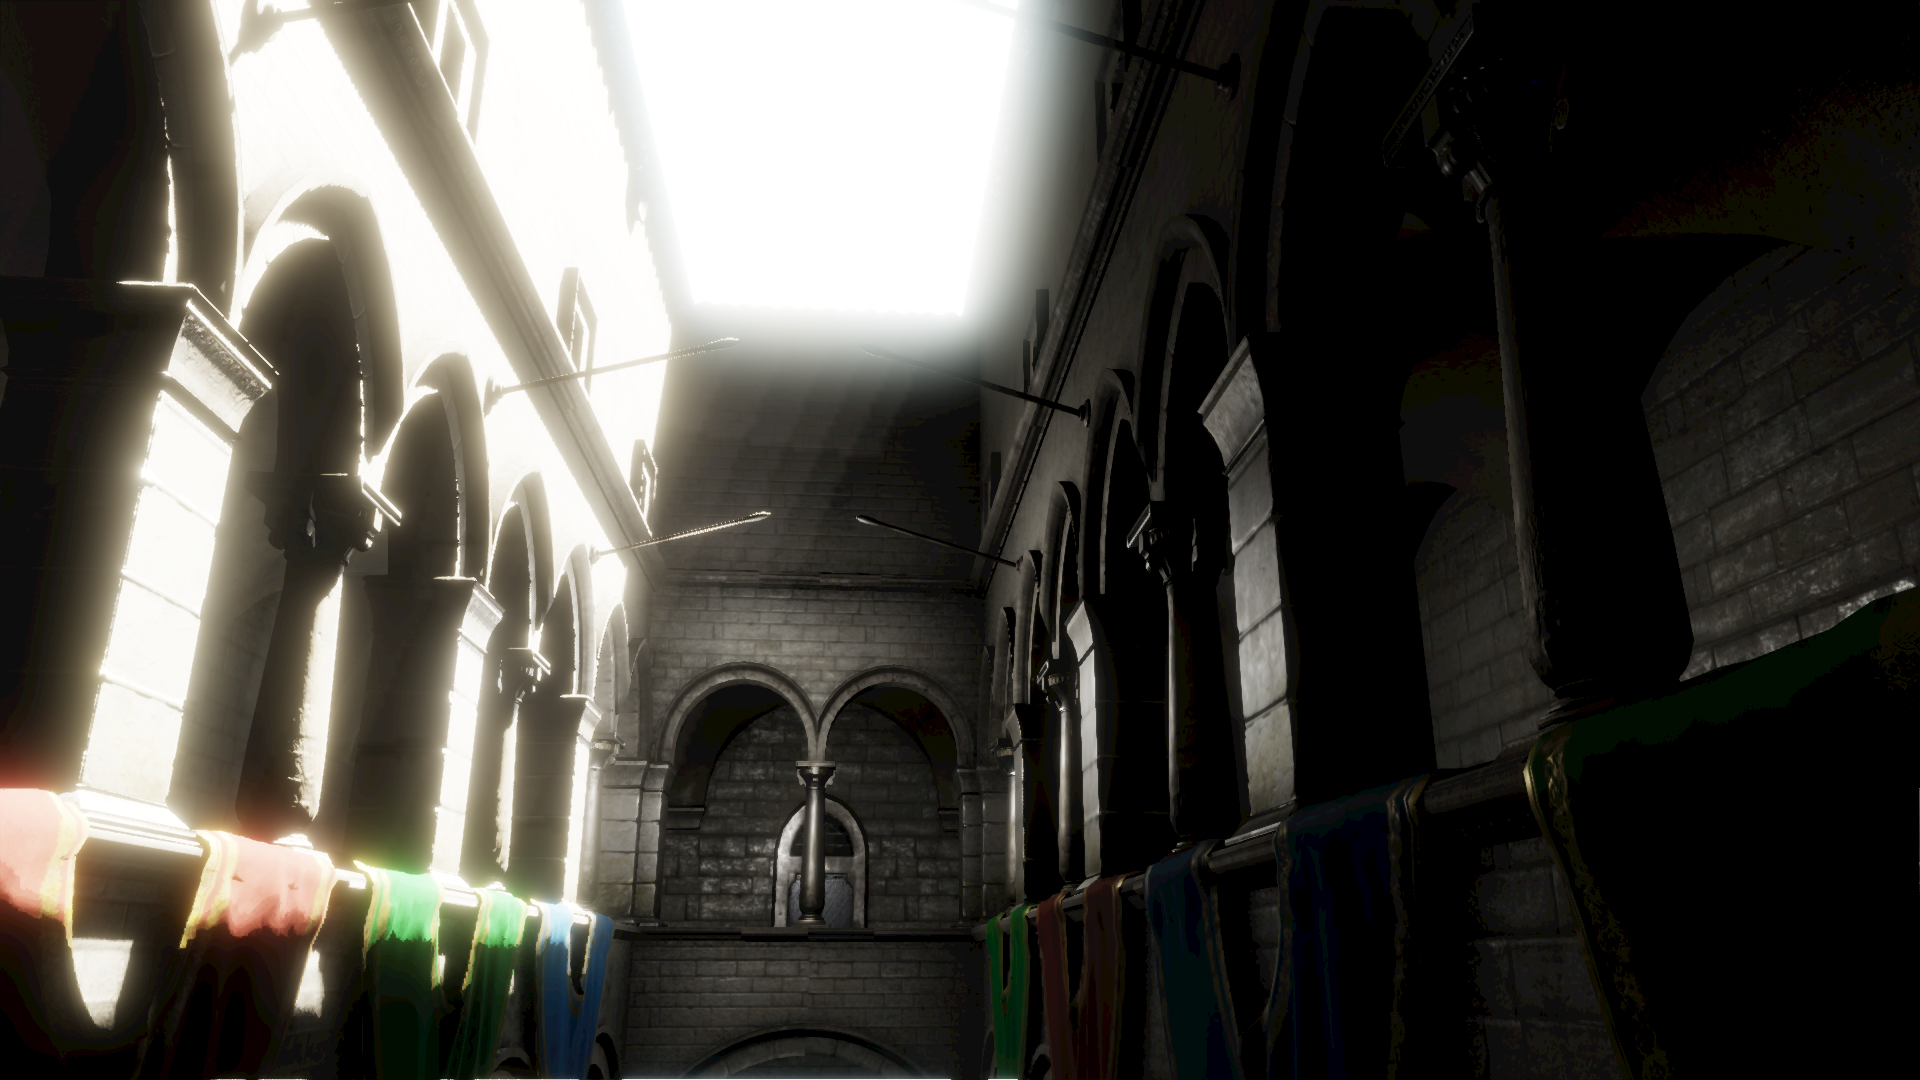
\includegraphics[width=\textwidth]{sunshaft_v2/mvp/frame_045.png}
    \caption{MVP 体积雾（轨迹中段，无深度保边）}
\end{subfigure}
\hfill
\begin{subfigure}{0.48\textwidth}
    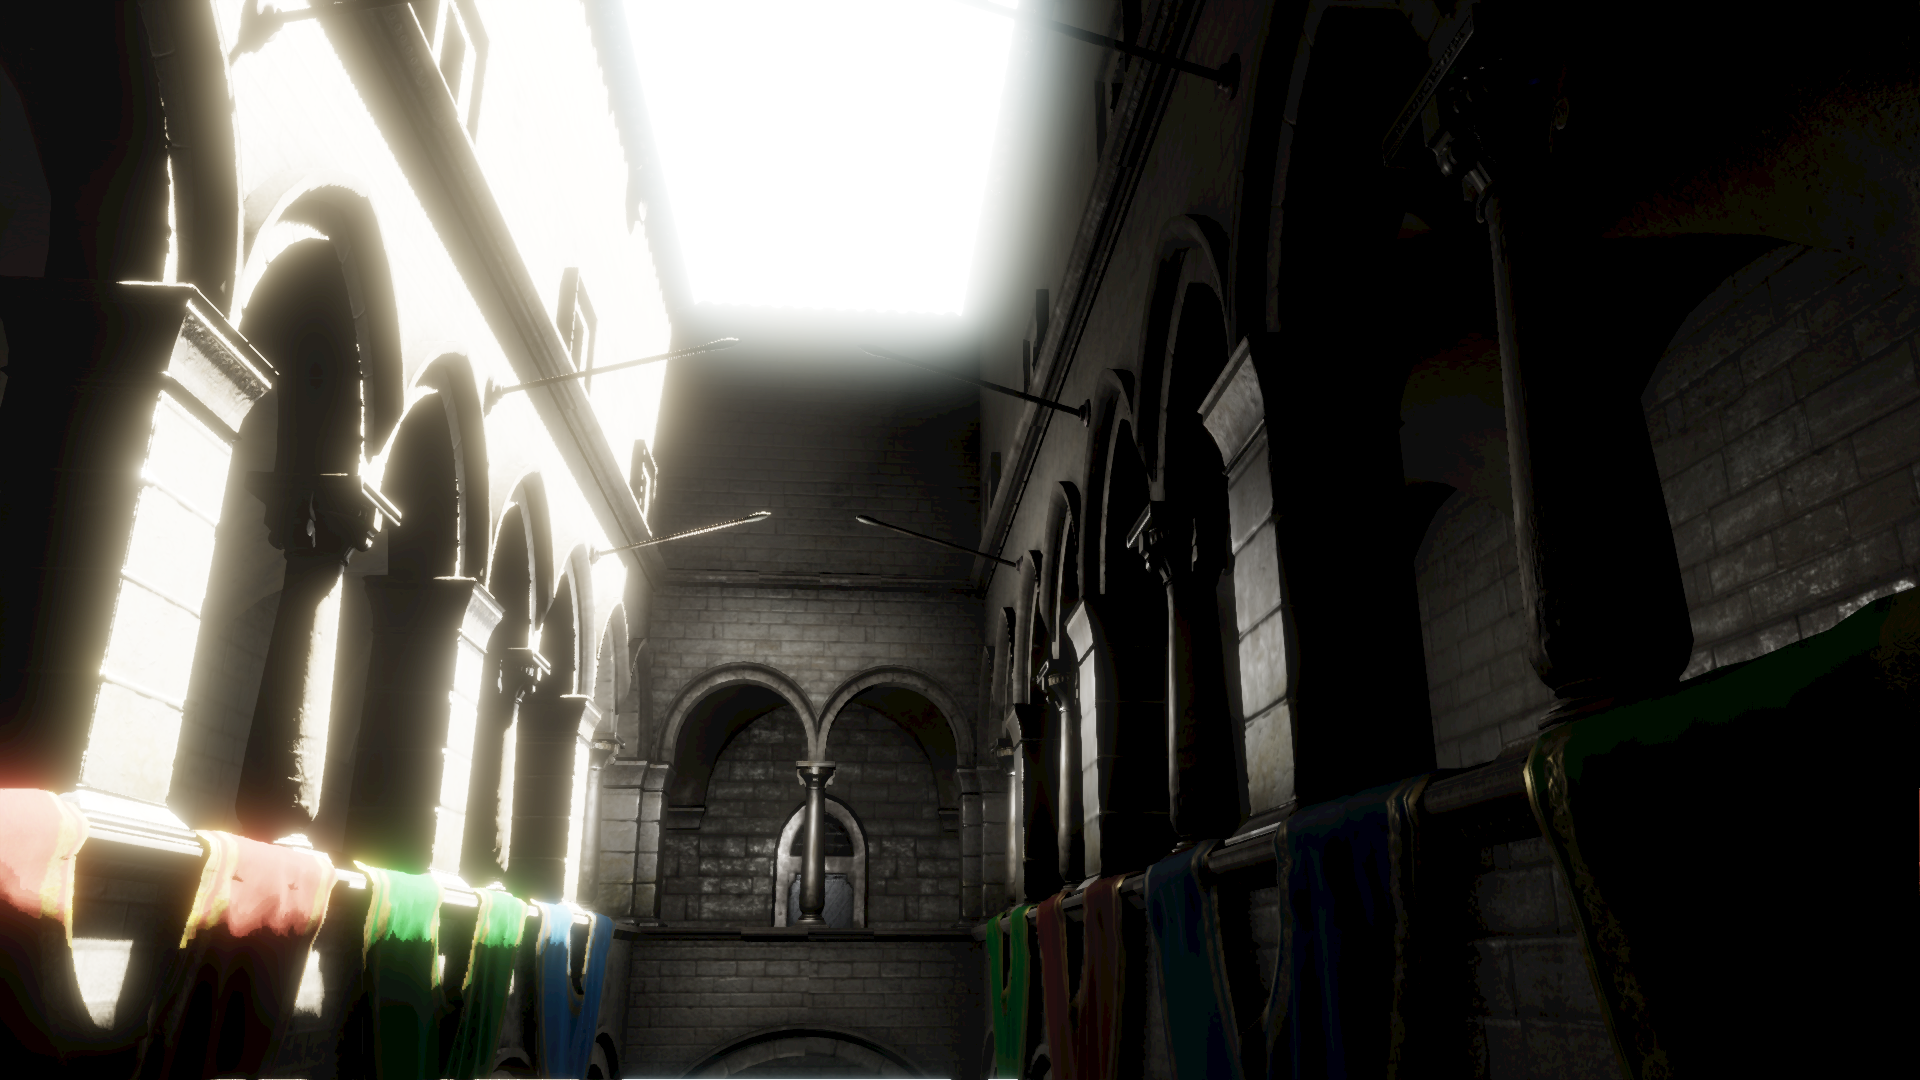
\includegraphics[width=\textwidth]{sunshaft_v2/halton/frame_045.png}
    \caption{优化后体积雾（轨迹中段，深度保边合成）}
\end{subfigure}
\caption{深度保边合成效果对比（frame 045）。左图 MVP 版本缺少深度引导权重，前景/背景深度断层处出现雾穿透几何轮廓的现象；右图优化后版本通过深度引导双线性插值和极薄轮廓回退机制，有效保留了柱体和帘布边缘。}
\label{fig:depth-aware-composite}
\end{figure}

% ================================================================
\section{动态 Probe GI 注入}
% ================================================================

\subsection{动机}

我们期望加入具有 MoerEngine 特性的优化，以提升体积雾渲染效果，通过调研以后，我们决定引入动态 Probe GI 注入。

UE 的体积雾使用烘焙或实时捕获的环境光作为低频边界辐射。MoerEngine 拥有独特的动态稀疏 Ray Query Probe GI 系统，它不依赖烘焙，可以在场景变化时实时更新方向辐照度。如果能将这套 Probe GI 接入体积雾，就能实现可随场景动态变化的间接雾光。

\subsection{工作组共享查询}

逐 Froxel 查询 Probe GI 的开销不可接受。利用 Compute Shader 的工作组共享内存，实现每 $4\times4\times4$ Froxel 工作组（64 个 Froxel）共享一次世界空间 Probe GI 查询：

\begin{lstlisting}[language=HLSL, caption={InjectDensity.hlsl 中的工作组共享 Probe GI 查询}]
const float3 group_world_position =
    stable_world_position_from_froxel(group_center, volume_size);

groupshared float4 group_probe_cache;
groupshared float4 group_probe_cache_meta;

// Only thread 0 in the group queries the radiance cache
if (all(dispatch_thread_id % 4 == 0)) {
    group_probe_cache = sample_group_probe_radiance(group_world_position, ...);
}
GroupMemoryBarrierWithGroupSync();

const float3 group_probe_radiance = group_probe_cache.rgb;
\end{lstlisting}

\subsection{四面体方向轮换}

Probe GI 使用球面四面体基进行方向重建。如果每个 Froxel 都查询同一方向，会导致方向偏差。解决方案是每帧将四面体方向旋转 $90^\circ$，在四帧内覆盖完整方向球面。这不新增体积缓存或 Dispatch，只改变查询方向参数。

% ================================================================
\section{FAST 采样论文适配}
% ================================================================

\subsection{论文选择过程}

在完成基础体积雾和 Probe GI 注入后，我期望能找一篇与 MoerEngine 架构相性匹配的采样论文，以此实现渲染效果的优化；在 AI 的帮助下，我们从近 3 年有关体积雾的研究中，选择了 FAST Froxel Jitter。最近两年的论文多数与深度学习相关，由于时间限制，我们很难在短时间内完成复现与模型的训练，因此我决定优先完成 FAST 的相关适配，而其他论文可以作为后期的研究方向。

\begin{table}[H]
\centering
\small
\begin{tabularx}{\textwidth}{lcccl}
\toprule
\textbf{候选方案} & \textbf{相性} & \textbf{研究价值} & \textbf{可实现性} & \textbf{结论} \\
\midrule
FAST Froxel Jitter & 5 & 5 & 4 & \textbf{本轮实施} \\
STBN Froxel Jitter & 3 & 5 & 3 & 作为 A/B 基线 \\
局部灯 ReSTIR & 3 & 4 & 4 & 后续研究 \\
神经多次散射 & 2 & 5 & 2 & 需 TensorRT \\
\bottomrule
\end{tabularx}
\caption{论文候选方案评分}
\end{table}

它具有如下优势：
\begin{enumerate}
    \item 它直接处理"全屏统一 Halton 空间相关"的问题，与 Moer 的 Froxel Jitter 完全对应；
    \item 它不增加新的 Render Pass、全分辨率纹理或 Ray Query；
    \item 它不破坏已有的稳定网格语义、CSM 稳定性和 Probe GI 查询；
\end{enumerate}

\subsection{FAST 原理简述}

FAST 的核心思想是：\textbf{采样器的误差不应只看单帧频谱，还应与实际的时间滤波器匹配}。传统 STBN（Spatio-Temporal Blue Noise）只优化蓝噪声频谱，但不知道引擎使用的是 0.94 历史权重、7-tap 非线性 Clamp 和动态历史拒绝。FAST 则根据这些滤波器参数生成更优的时空样本。

\subsection{工程化适配}

\subsubsection{FAST 噪声纹理}

使用公开生成器生成的 \texttt{Vector3} FAST 纹理，参数为 \texttt{gauss1\_exp006\_beta010}：

\begin{itemize}
    \item 尺寸：$64\times64\times32$（空间 XY + 时间 Z），RGBA8 格式
    \item 显存：$64\times64\times32\times4 = 524{,}288$ 字节 $\approx 0.5$\,MiB
    \item 选择 \texttt{Vector3} 而非三张独立标量纹理：让 XYZ 联合样本空间也参与优化
    \item 选择 RGBA8 而非浮点格式：Jitter 的量化误差远小于 Froxel 尺寸
\end{itemize}

\subsubsection{C++ 加载与回退}

\begin{lstlisting}[language=cppinline, caption={VolumetricFogPass.cpp 中的 FAST 纹理加载}]
static constexpr std::string_view fast_noise_filename =
    "volumetric_fog_fast_vector3_gauss1_exp006_beta010_64x64x32.rgba8";

// If FAST texture is unavailable, silently fall back to Halton
if (IsFastNoiseMode(active_jitter_mode) && !fast_noise_ready) {
    active_jitter_mode = EVolumetricFogJitterMode::HALTON;
    LOG_WARNING("[VolumetricFog][FAST] Noise unavailable; using Halton fallback.");
}
\end{lstlisting}

\subsubsection{Shader 采样}

\begin{lstlisting}[language=HLSL, caption={InjectDensity.hlsl 中的 FAST 采样}]
uint noise_width, noise_height, noise_frames;
fast_noise_texture.GetDimensions(noise_width, noise_height, noise_frames);
const uint frame = param.jitter_frame_index % max(noise_frames, 1u);
const uint cycle = param.jitter_frame_index / max(noise_frames, 1u);

// FAST is optimized on a torus. Integer offsets preserve the stored
// sample values and the intra-frame spectrum, while extending a finite
// time cycle without re-hashing the samples.
uint2 offset = uint2(fog_hash(cycle ^ 0x9e3779b9u),
                      fog_hash(cycle ^ 0x243f6a88u));
if (param.jitter_mode == FAST_XYZ_OFFSET) {
    offset += uint2(froxel_id.z * 37u, froxel_id.z * 17u);
}
const uint2 coordinate = uint2(
    (froxel_id.x + offset.x) % max(noise_width, 1u),
    (froxel_id.y + offset.y) % max(noise_height, 1u)
);
return fast_noise_texture.Load(int4(coordinate, frame, 0)).rgb - 0.5;
\end{lstlisting}

关键设计：FAST 在环面（torus）上优化，通过整数偏移扩展有限时间周期，保持存储样本值和帧内频谱不变。

\subsubsection{两种 FAST 模式}

\begin{itemize}
    \item \textbf{FAST\_XY}：仅在 XY 方向使用 FAST 纹理采样，Z 方向仍使用 Halton
    \item \textbf{FAST\_XYZ\_OFFSET}：在 XY 基础上，按 Z 层额外偏移，扩展空间去相关
\end{itemize}

\begin{figure}[H]
\centering
\begin{subfigure}{0.48\textwidth}
    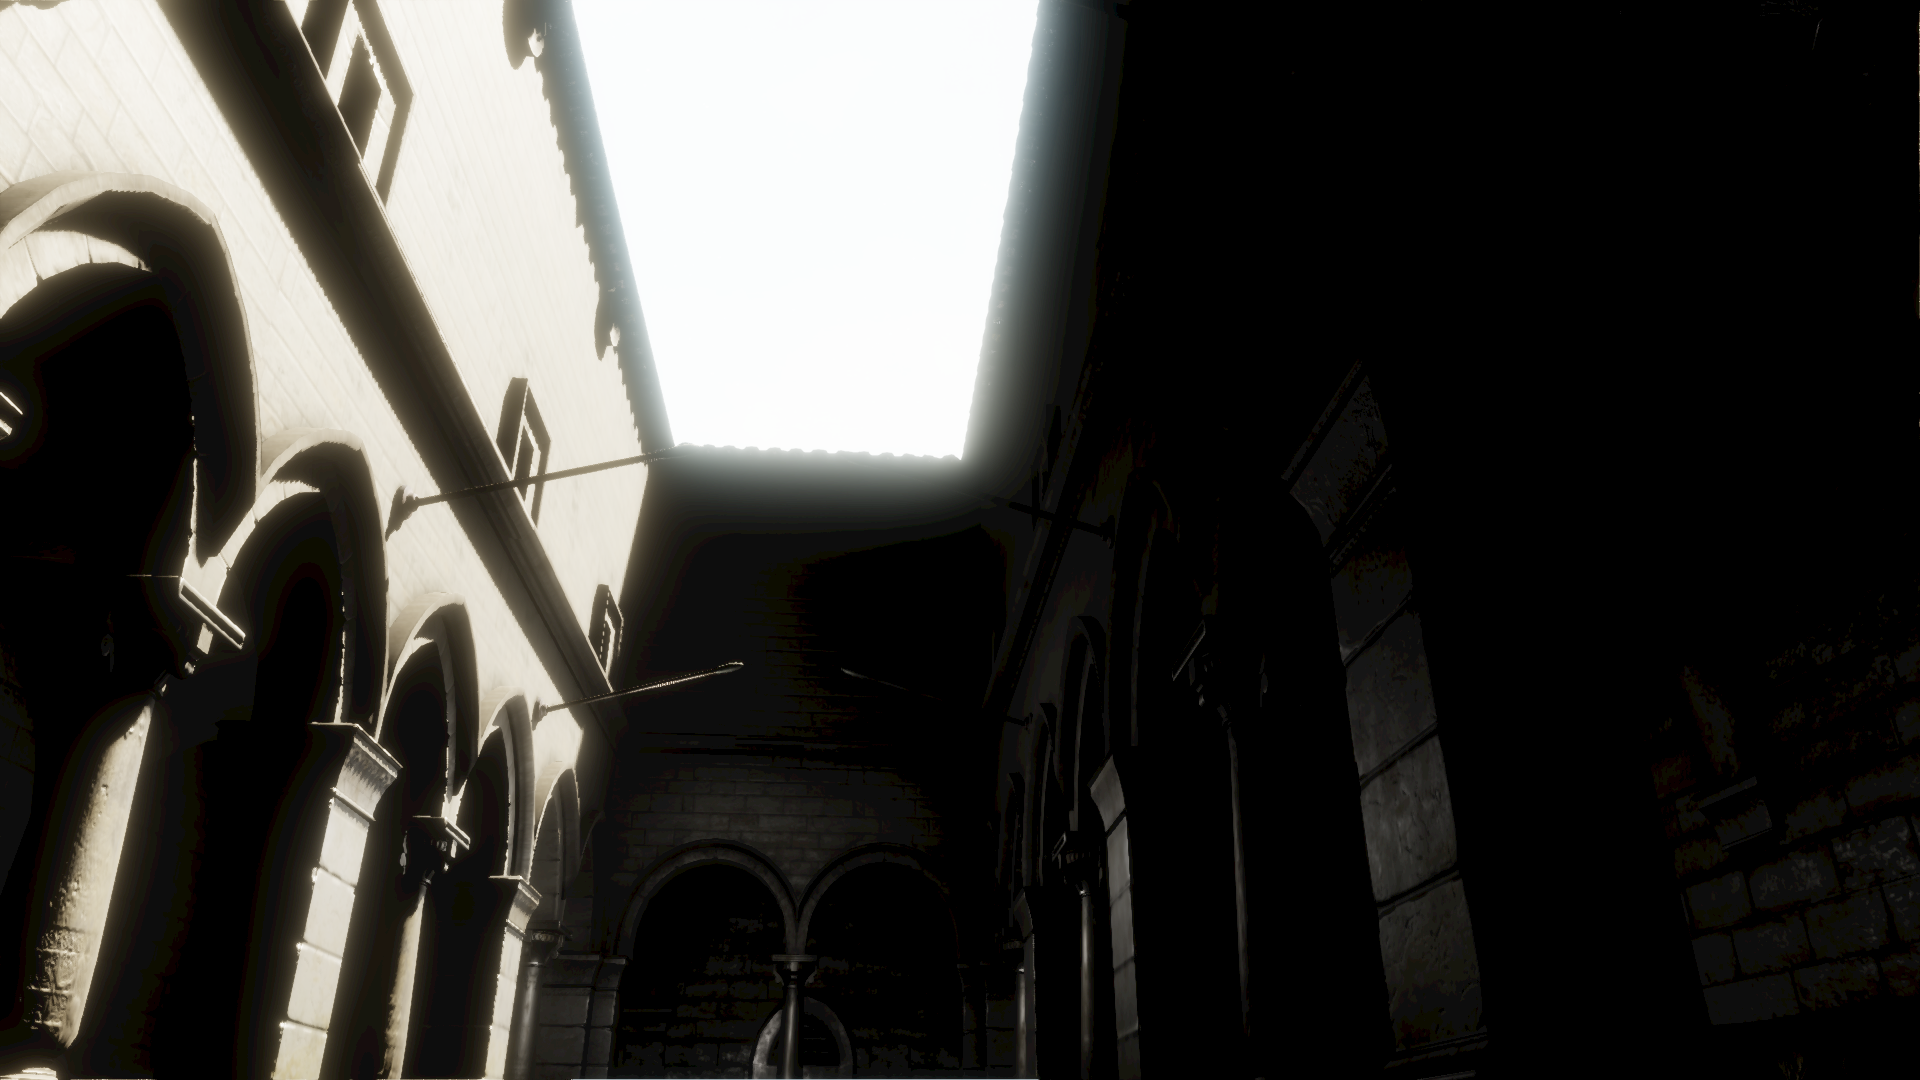
\includegraphics[width=\textwidth]{sunshaft_v2/halton/frame_089.png}
    \caption{Halton 基线（轨迹终点 frame 89）}
\end{subfigure}
\hfill
\begin{subfigure}{0.48\textwidth}
    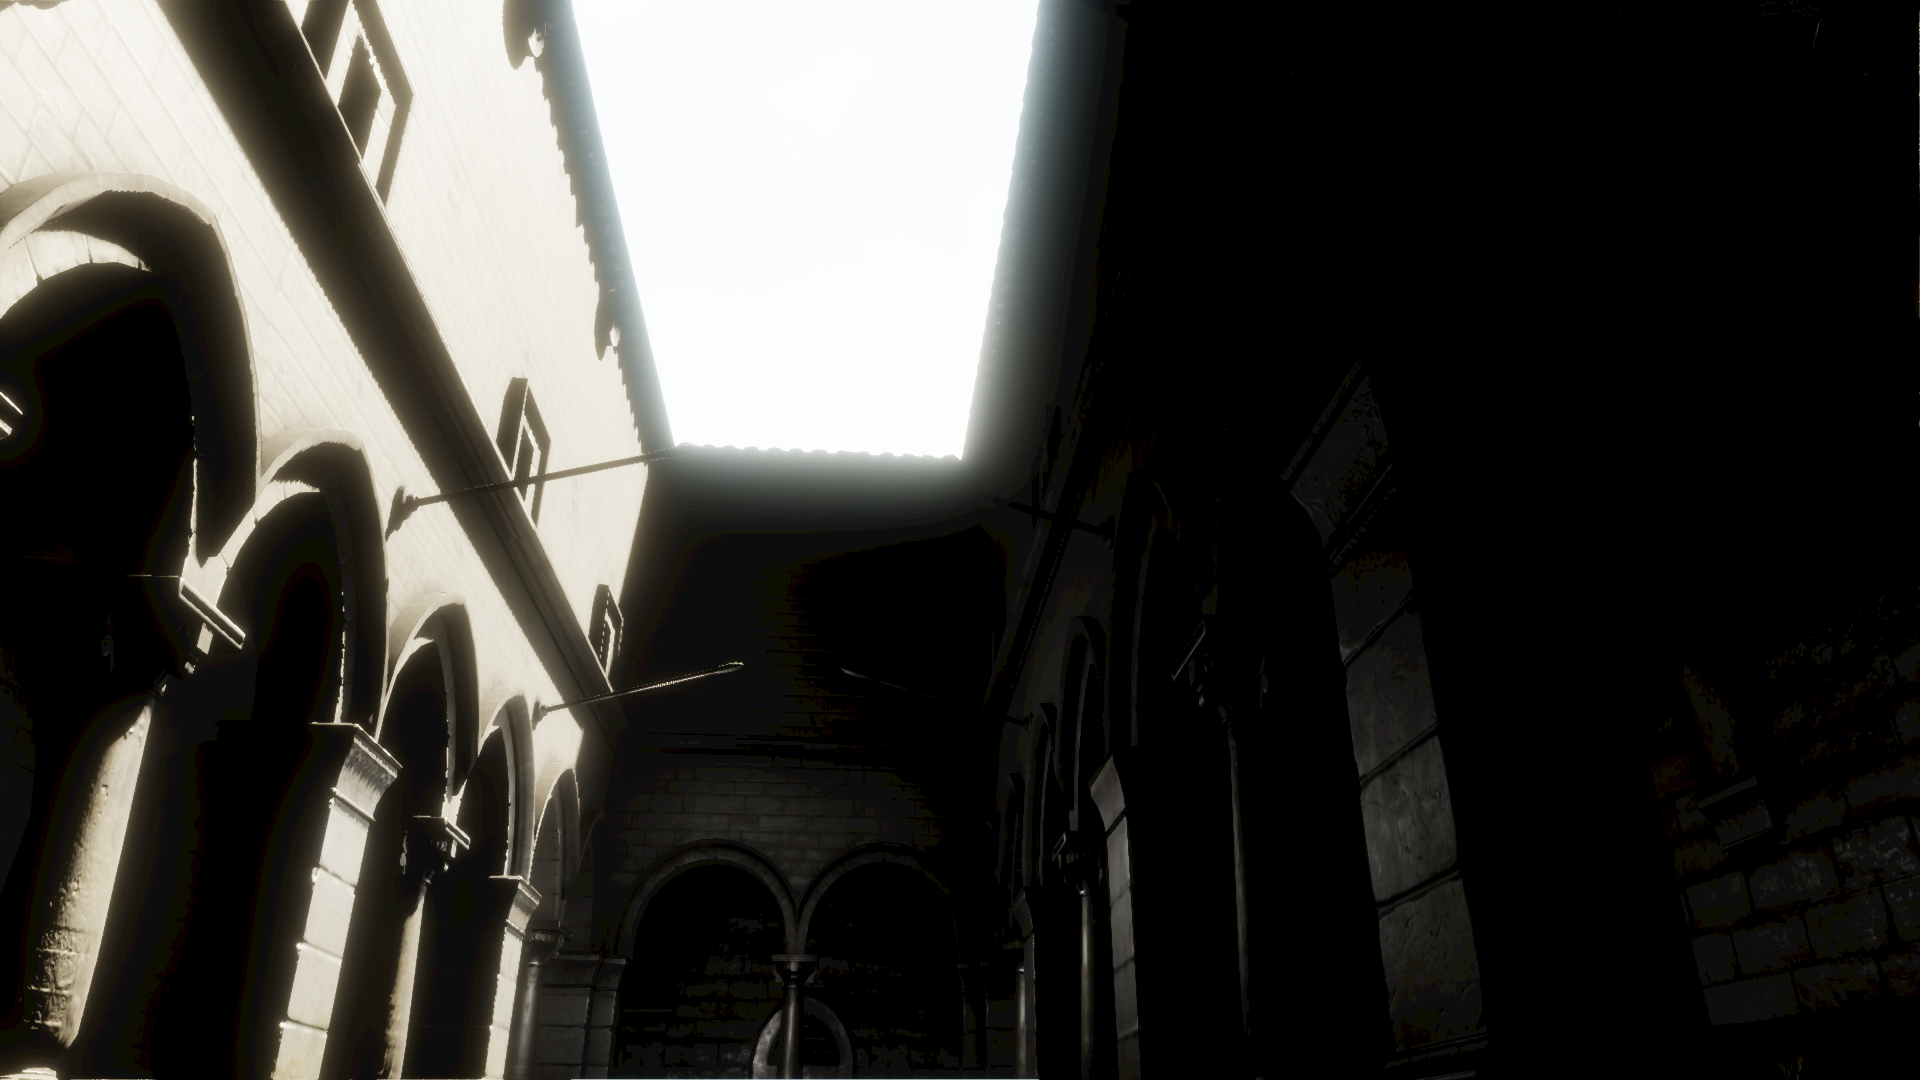
\includegraphics[width=\textwidth]{sunshaft_v2/fast_xy/frame_089.png}
    \caption{FAST XY（轨迹终点 frame 89）}
\end{subfigure}
\caption{Halton 与 FAST XY 采样在轨迹终点的静止收敛对比。两者画面接近，未观察到新的固定图案或明显层带。}
\label{fig:fast-comparison}
\end{figure}

\subsubsection{像素差异量化}

\begin{table}[H]
\centering
\small
\begin{tabular}{rrrrrr}
\toprule
帧 & 默认密度 YAVG & 默认密度 YMAX & 高对比度 YAVG & 高对比度 YMAX & 差异倍数 \\
\midrule
0 & 0.008 & 2 & 0.160 & 8 & 20$\times$ \\
10 & 0.008 & 1 & 0.147 & 6 & 18$\times$ \\
30 & 0.008 & 1 & 0.140 & 7 & 18$\times$ \\
45 & 0.022 & 4 & 0.092 & 4 & 4$\times$ \\
75 & 0.011 & 2 & 0.049 & 4 & 4$\times$ \\
89 & 0.004 & 1 & 0.053 & 4 & 14$\times$ \\
\bottomrule
\end{tabular}
\caption{Halton 与 FAST XY 的帧级像素差异（YAVG = 平均亮度差/255，YMAX = 最大亮度差/255）}
\end{table}

\subsubsection{未收敛场景对比}

上述对比均在 120 帧 warmup 后（时域已收敛）进行。但实际游戏中，相机切换、快速转头或进入新区域时，历史会失效，体积雾需要从零重建。为模拟这一场景，使用 \texttt{nocoverage} preset：

\begin{itemize}
    \item \textbf{warmup 仅 10 帧}（而非 120 帧），捕获时域尚未收敛的前几帧
    \item \textbf{history\_weight = 0.50}（而非 0.94），每帧采样贡献更大，收敛更慢
    \item \textbf{高密度 + 陡梯度}（与 highcontrast 相同的介质参数）
\end{itemize}

\begin{table}[H]
\centering
\small
\begin{tabular}{rrrrrr}
\toprule
帧 & 收敛场景 YAVG & 收敛场景 YMAX & 未收敛 YAVG & 未收敛 YMAX & 增大倍数 \\
\midrule
0 & 0.160 & 8 & 0.002 & 1 & --- \\
10 & 0.147 & 6 & 0.018 & 4 & 8$\times$ \\
20 & --- & --- & 0.069 & 5 & --- \\
30 & 0.140 & 7 & 0.111 & 9 & --- \\
45 & 0.092 & 4 & 0.200 & \textbf{12} & 2$\times$ \\
60 & --- & --- & 0.177 & 7 & --- \\
75 & 0.049 & 4 & \textbf{0.278} & 7 & \textbf{6$\times$} \\
89 & 0.053 & 4 & 0.100 & 7 & 2$\times$ \\
\bottomrule
\end{tabular}
\caption{未收敛场景与收敛场景的 Halton vs FAST 像素差异对比}
\end{table}

% ================================================================
\section{自适应稀疏体积辐射缓存 (VRC)}
% ================================================================

\subsection{动机与定位}

Froxel 体积雾的视锥网格只能覆盖相机附近的有限范围。对于远处的间接雾光，需要一个稳定的世界空间缓存。UE 使用烘焙的体积光照贴图（VLM），但 Moer 没有烘焙管线。针对 MoerEngine 的在线引擎特点，我们使用了 VRC（Volume Radiance Cache）来存储世界空间缓存。

Moer 的动态稀疏 Probe GI 已经拥有完整的 Cell $\to$ Brick $\to$ Page Table $\to$ Streaming $\to$ Dirty Tracking 基础设施。VRC 的思路是\textbf{复用这套稀疏层级，存储独立的参与介质辐射数据}。

\subsection{自适应稀疏布局与调度}

VRC 复用 Probe GI 的 Volume $\to$ Cell $\to$ Brick $\to$ Page Table 结构，但加入了\textbf{介质感知}的细化调度：

\begin{enumerate}
    \item 对每个 Probe Cell 采样中心与 8 个角点，估计全局指数高度雾和局部球形雾的平均密度
    \item 计算相对密度梯度、屏幕贡献和介质优先级
    \item 将介质期望层级与原有几何期望层级合并；高密度、高梯度或高屏幕贡献区域优先细化
    \item 更新调度在 mandatory/dirty 优先级之后加入介质优先级和更新年龄，受每帧 Brick 预算约束
\end{enumerate}

\begin{table}[H]
\centering
\begin{tabular}{lrl}
\toprule
参数 & 默认值 & 作用 \\
\midrule
Density Threshold & 0.0010 & 判断 Cell 是否需要体积缓存 \\
Gradient Threshold & 0.18 & 密度变化较大时细化 \\
Screen Weight & 1.0 & 屏幕贡献权重 \\
Priority Weight & 2.0 & 更新调度中的介质优先级权重 \\
History Weight & 0.88 & 双缓冲历史融合 \\
Multi Scatter & 0.12 & 受控的近似高阶散射反馈 \\
Transmittance Steps & 6 & 介质光学深度积分步数 (2--12) \\
\bottomrule
\end{tabular}
\caption{VRC 自适应调度参数}
\end{table}

\subsection{独立 L1 方向辐射缓存}

每个物理 Probe 保存 L0（各向同性）和 L1-X/Y/Z（一阶方向性）：

\begin{equation}
L(\mathbf{d}) = L_0 + L_{1x} \cdot d_x + L_{1y} \cdot d_y + L_{1z} \cdot d_z
\end{equation}

\begin{itemize}
    \item 最多 2048 个物理 Probe，单份缓存 163,840 字节
    \item 采用 history/write 双缓冲，更新前复制未调度记录，随后只覆盖本帧稀疏 Brick
    \item 双缓冲共 327,680 字节 $\approx$ \textbf{0.3125\,MiB}，没有新增密集 3D 辐射纹理
\end{itemize}

\subsection{介质感知传输}

\subsubsection{直接光散射源}

第一阶直接光先转换为介质散射源再缓存，避免在 Froxel 注入阶段重复计算一次散射：

\begin{equation}
L_{\text{direct}} = \sum_{\text{lights}} \Phi_{\text{light}} \cdot V_{\text{RayQuery}} \cdot T_{\text{medium}} \cdot \sigma_{\text{scat}} \cdot p(\theta)
\end{equation}

其中 $V_{\text{RayQuery}}$ 是通过硬件 Ray Query 对不透明几何执行的可见性测试，$T_{\text{medium}}$ 是沿光线 2--12 步的 Beer-Lambert 透射率积分。

\subsubsection{历史邻域多次散射}

从上一帧缓存采样 6 个邻居，按透射率衰减提供受控的近似多次散射反馈：

\begin{lstlisting}[language=HLSL, caption={UpdateRadianceCache.hlsl 中的邻域多次散射}]
const float transmittance = integrate_medium_transmittance(
    current_position,
    safe_normalize(neighbor.world_position.xyz - current_position, float3(0,1,0)),
    distance
);
radiance_sum += max(neighbor.l0.rgb, 0.0) * transmittance * saturate(neighbor.l0.w);
weight_sum += saturate(neighbor.l0.w);
\end{lstlisting}

\begin{figure}[H]
\centering
\begin{subfigure}{0.48\textwidth}
    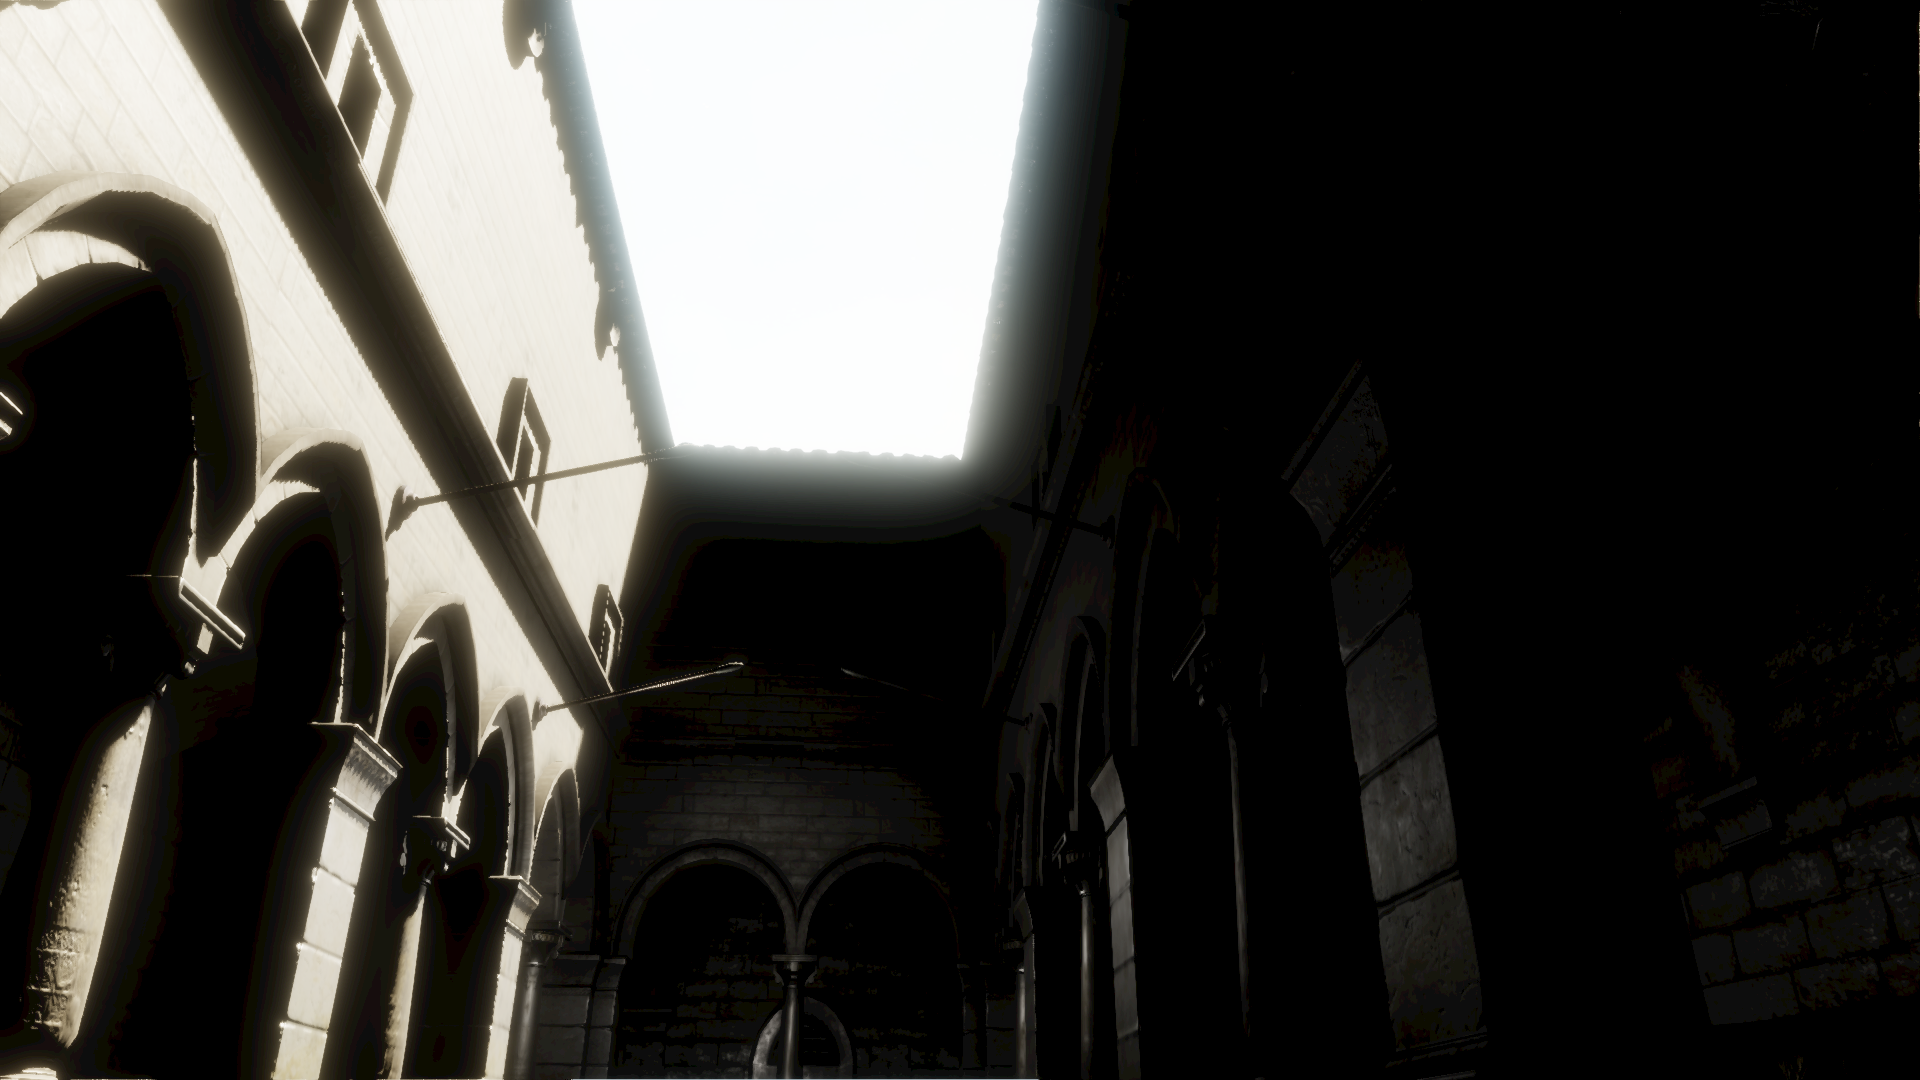
\includegraphics[width=\textwidth]{sunshaft_v2/off/frame_089.png}
    \caption{无体积雾（轨迹终点）}
\end{subfigure}
\hfill
\begin{subfigure}{0.48\textwidth}
    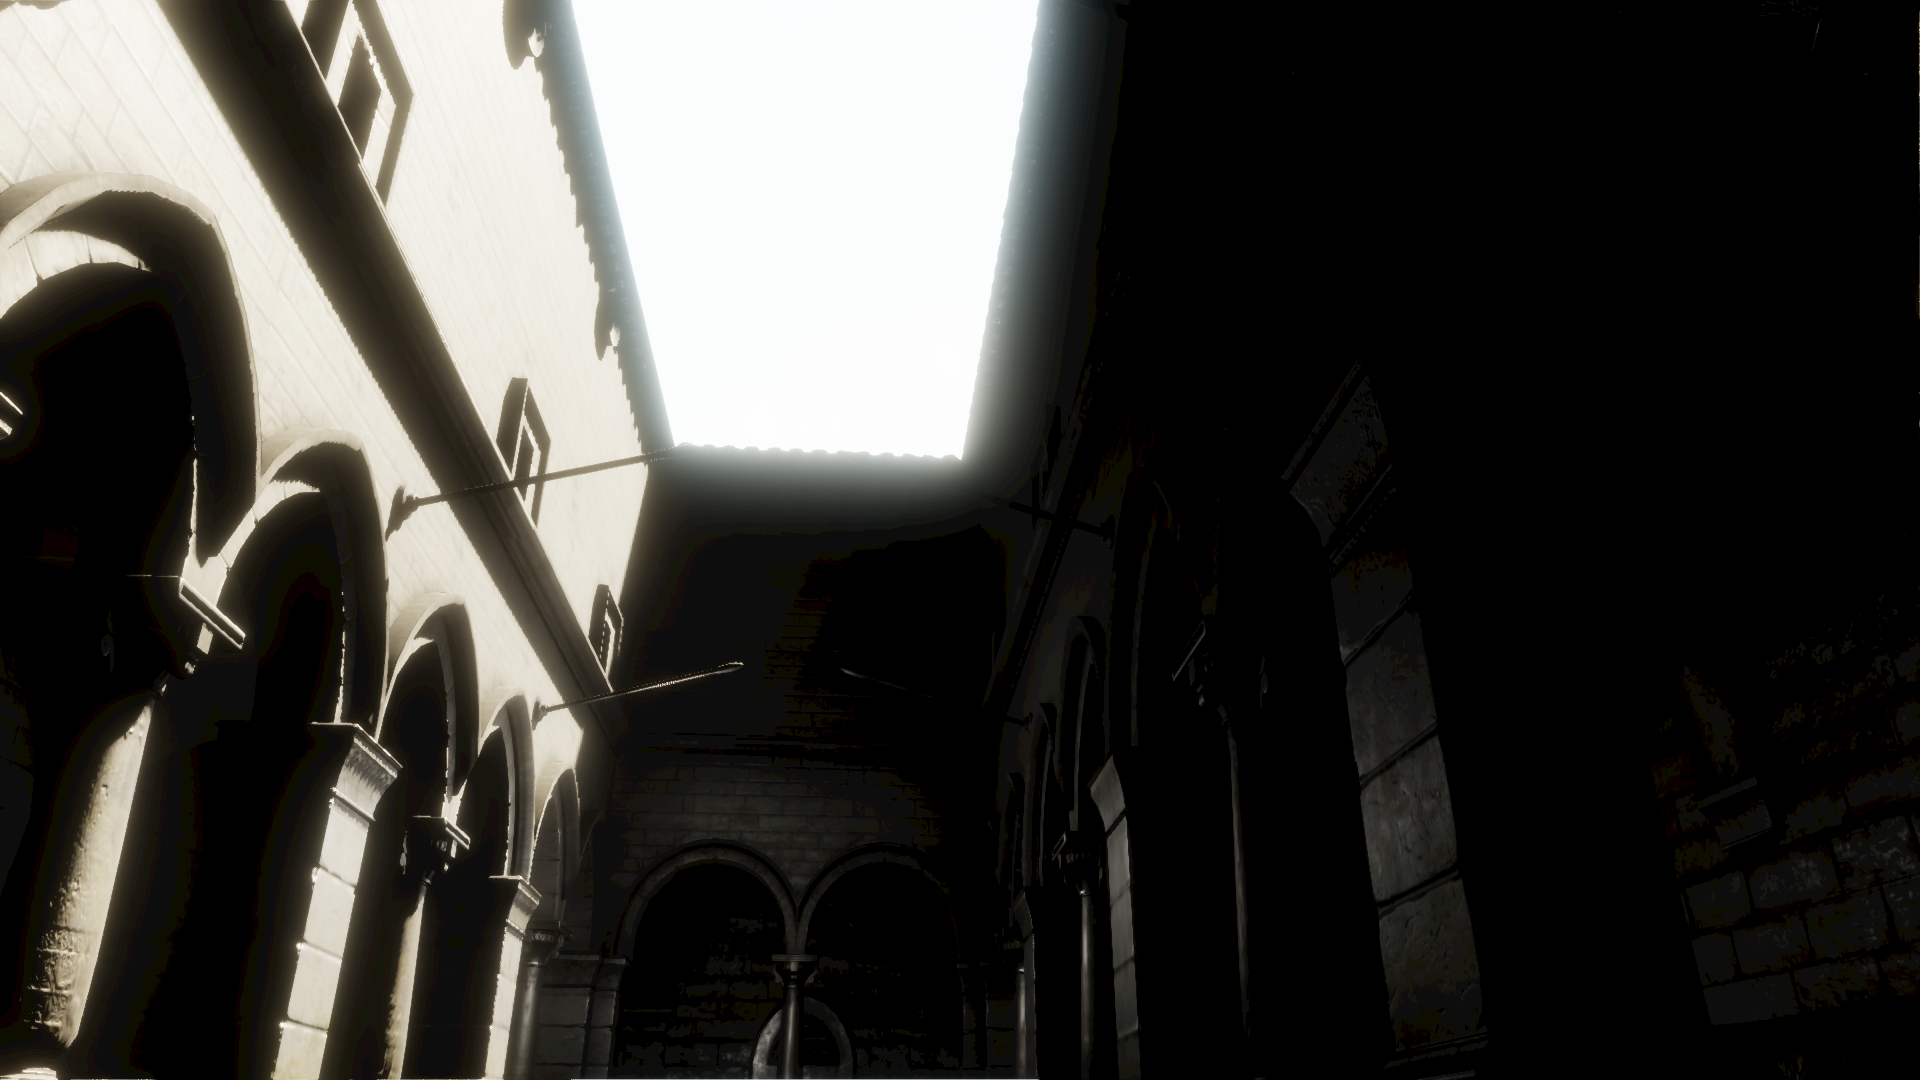
\includegraphics[width=\textwidth]{sunshaft_v2/mvp/frame_089.png}
    \caption{MVP 体积雾（轨迹终点）}
\end{subfigure}

\vspace{0.3cm}

\begin{subfigure}{0.48\textwidth}
    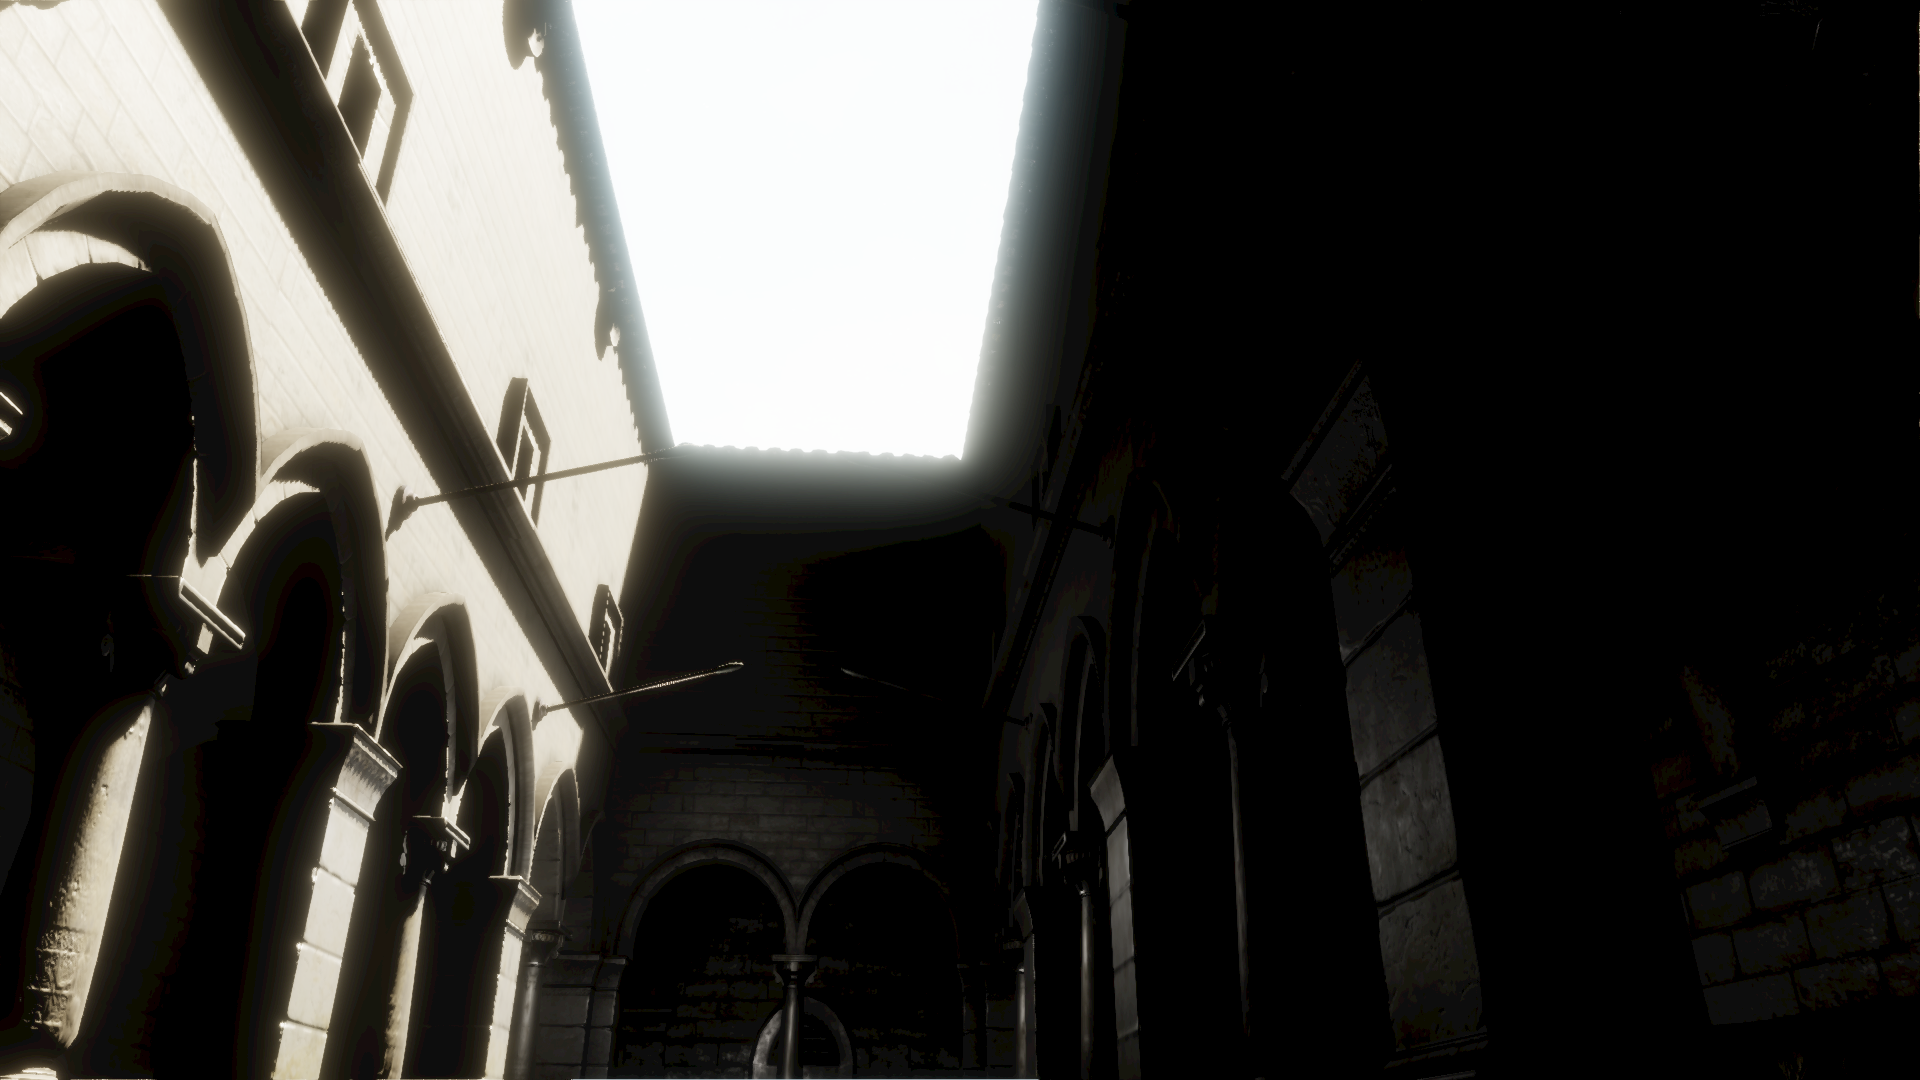
\includegraphics[width=\textwidth]{sunshaft_v2/halton/frame_089.png}
    \caption{优化后体积雾（轨迹终点）}
\end{subfigure}
\hfill
\begin{subfigure}{0.48\textwidth}
    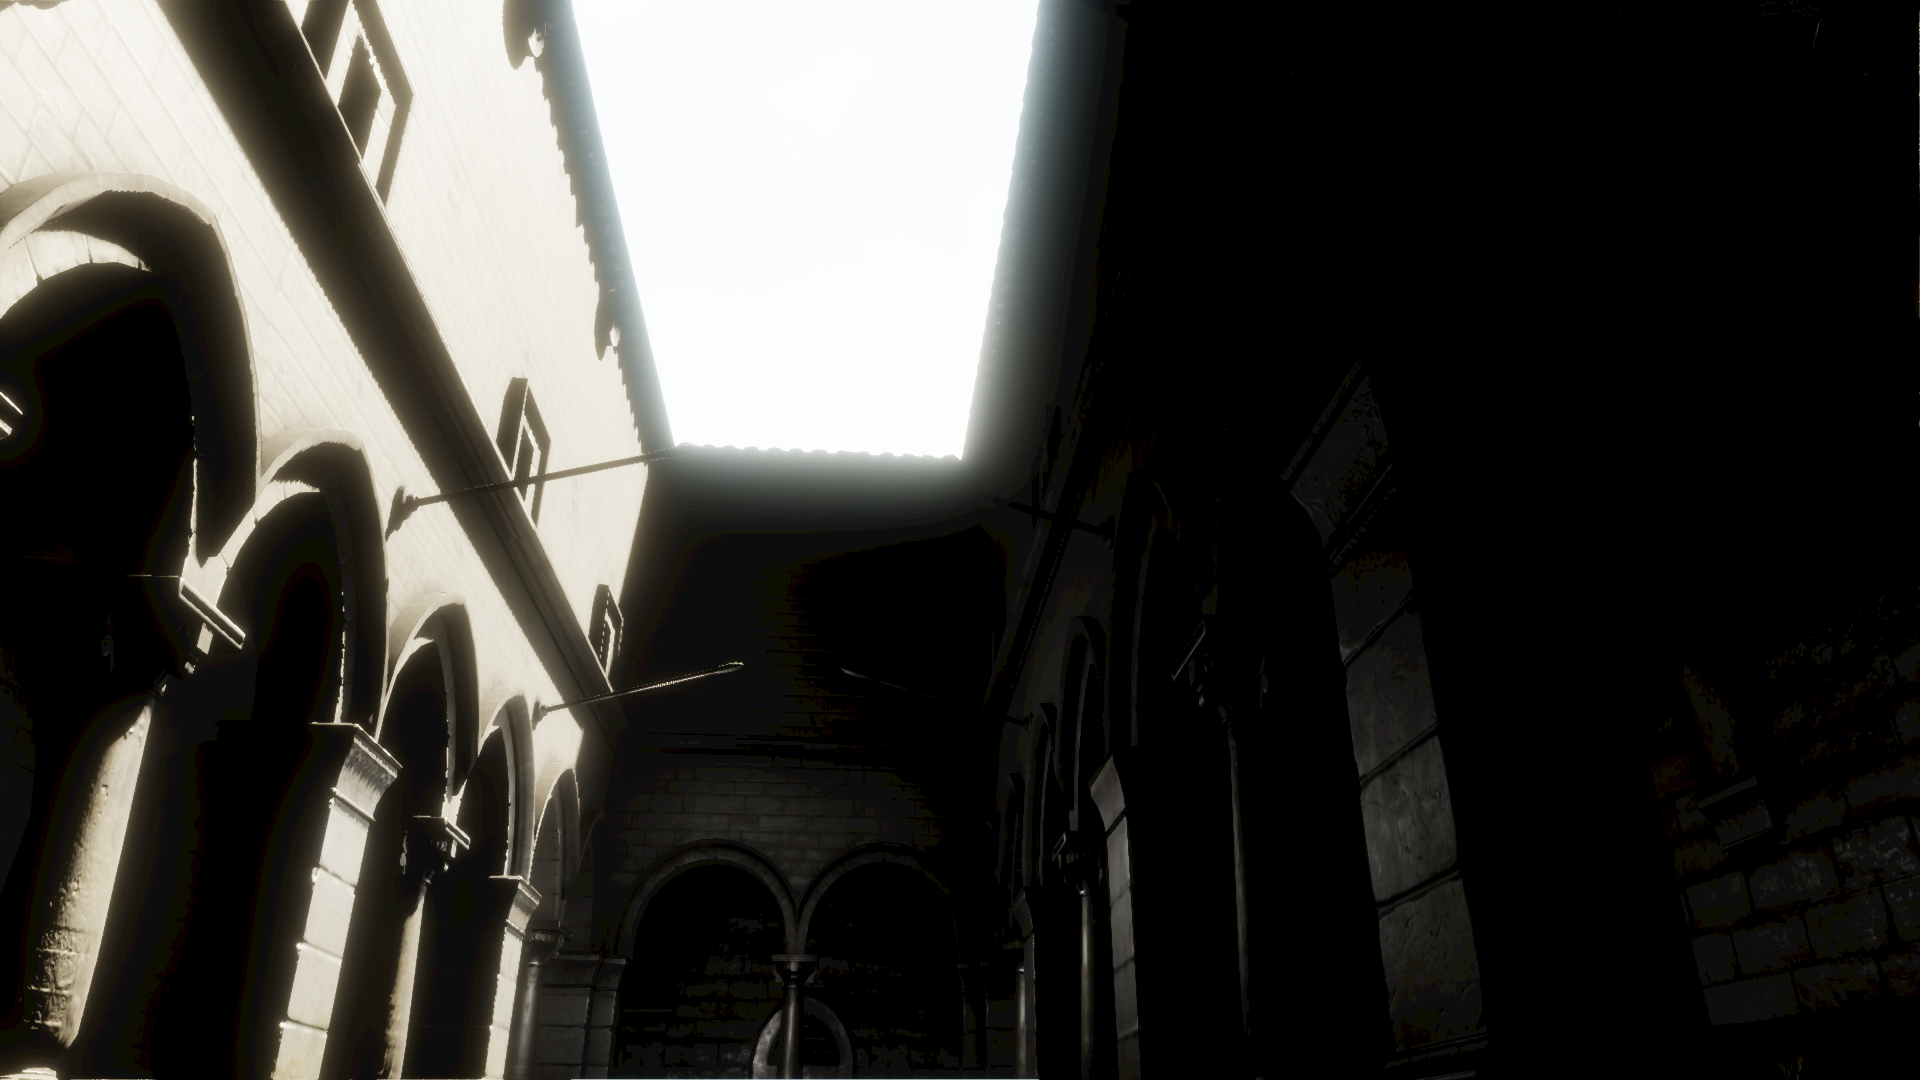
\includegraphics[width=\textwidth]{sunshaft_v2/fast_xy/frame_089.png}
    \caption{FAST 体积雾（轨迹终点）}
\end{subfigure}
\caption{四种状态在 Benchmark 轨迹终点（frame 89）的对比。优化后和 FAST 版本均开启 Probe GI + VRC，暗区获得彩色间接雾光。}
\label{fig:four-state-end}
\end{figure}

% ================================================================
\section{性能实测与效果展示}
% ================================================================

\subsection{效果展示}

\begin{figure}[H]
\centering
\begin{subfigure}{0.48\textwidth}
    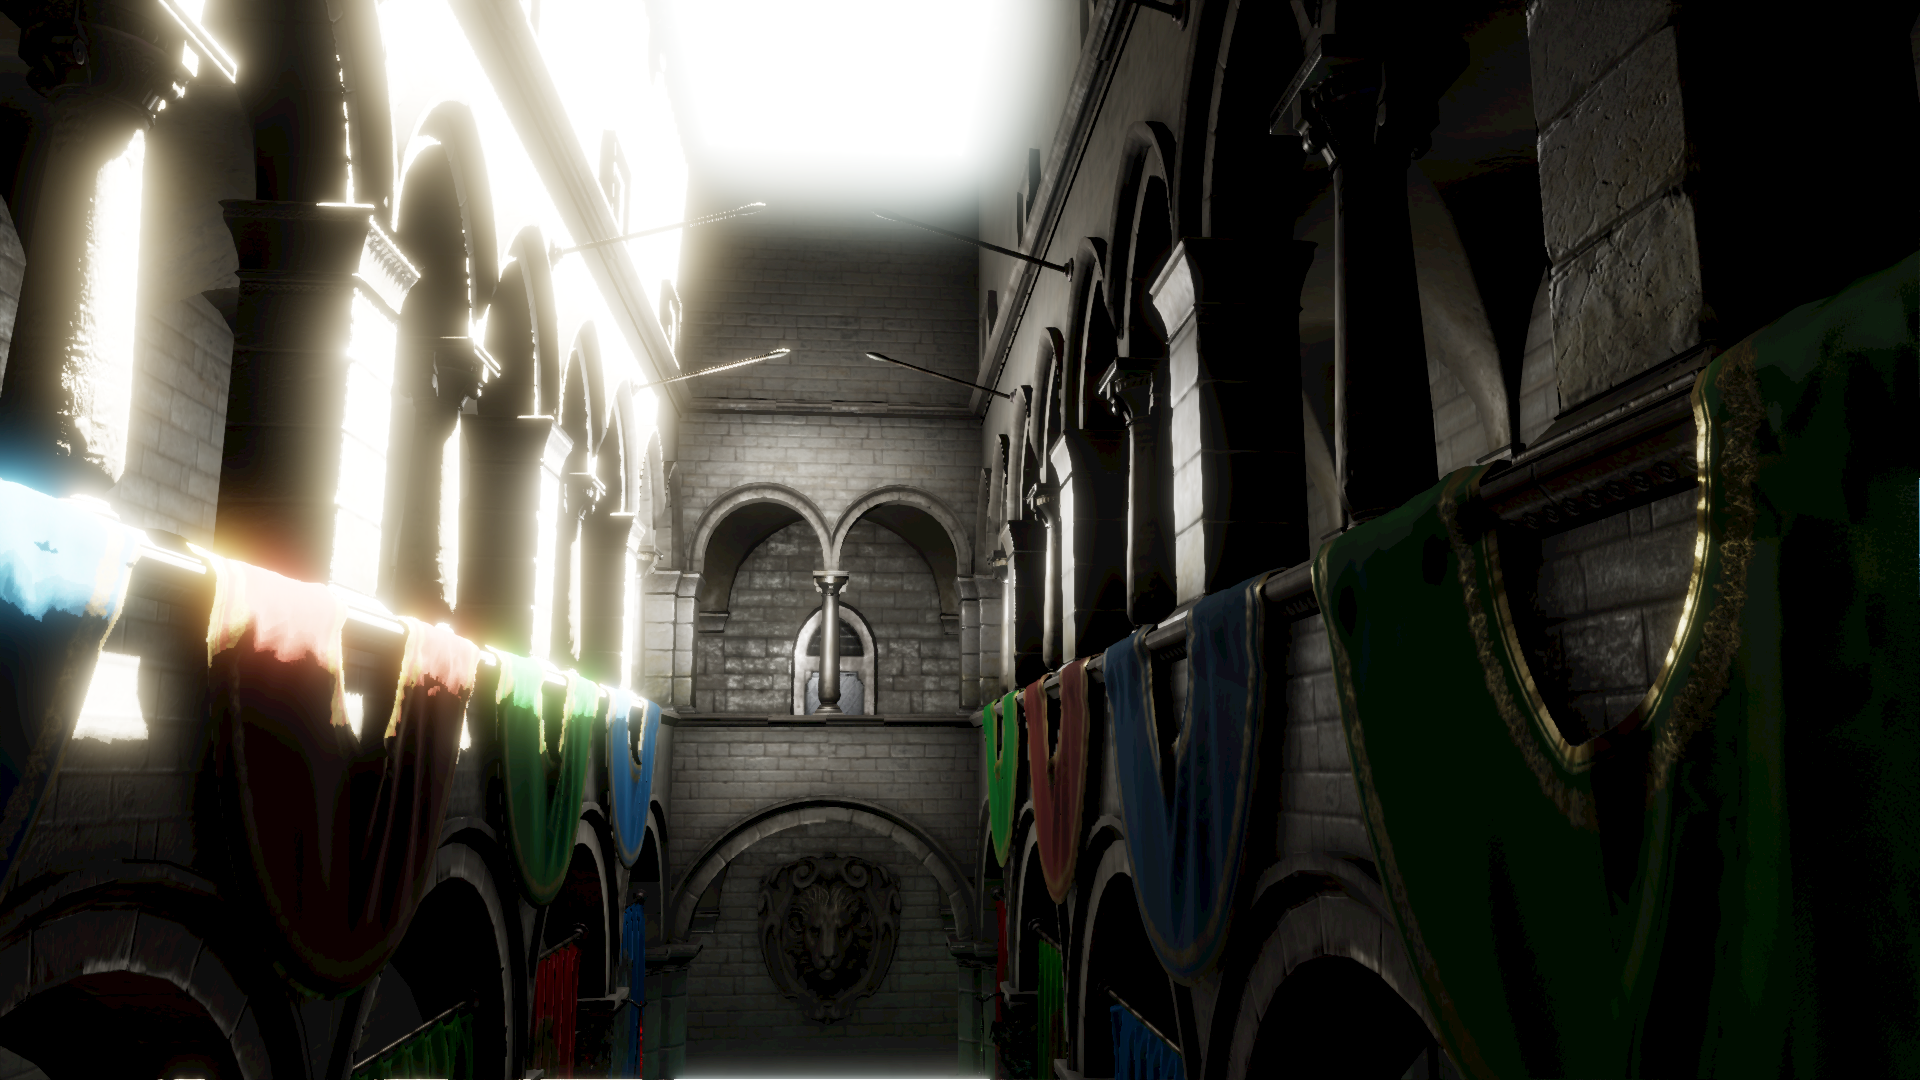
\includegraphics[width=\textwidth]{sunshaft_v2/off/frame_000.png}
    \caption{无体积雾（\texttt{off}）}
\end{subfigure}
\hfill
\begin{subfigure}{0.48\textwidth}
    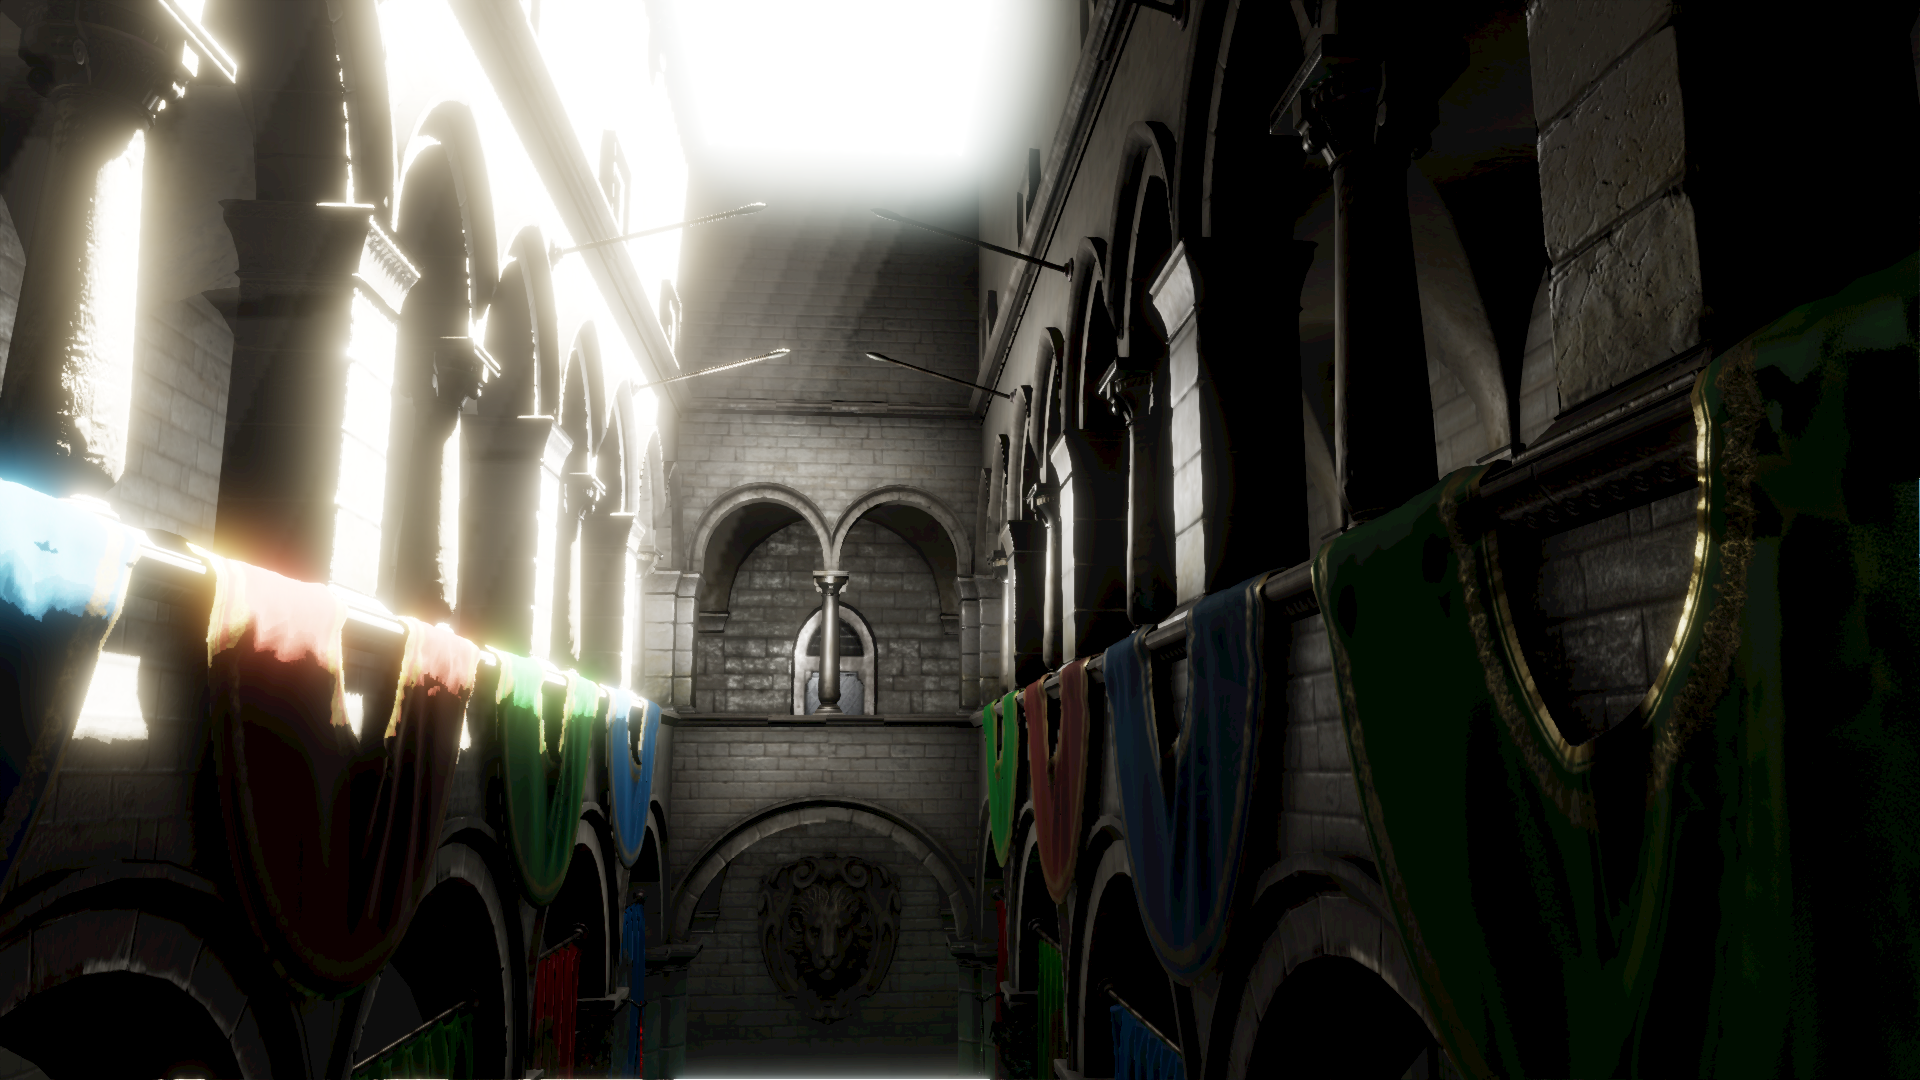
\includegraphics[width=\textwidth]{sunshaft_v2/mvp/frame_000.png}
    \caption{MVP 体积雾（\texttt{mvp}：无时域、PCF0）}
\end{subfigure}

\vspace{0.3cm}

\begin{subfigure}{0.48\textwidth}
    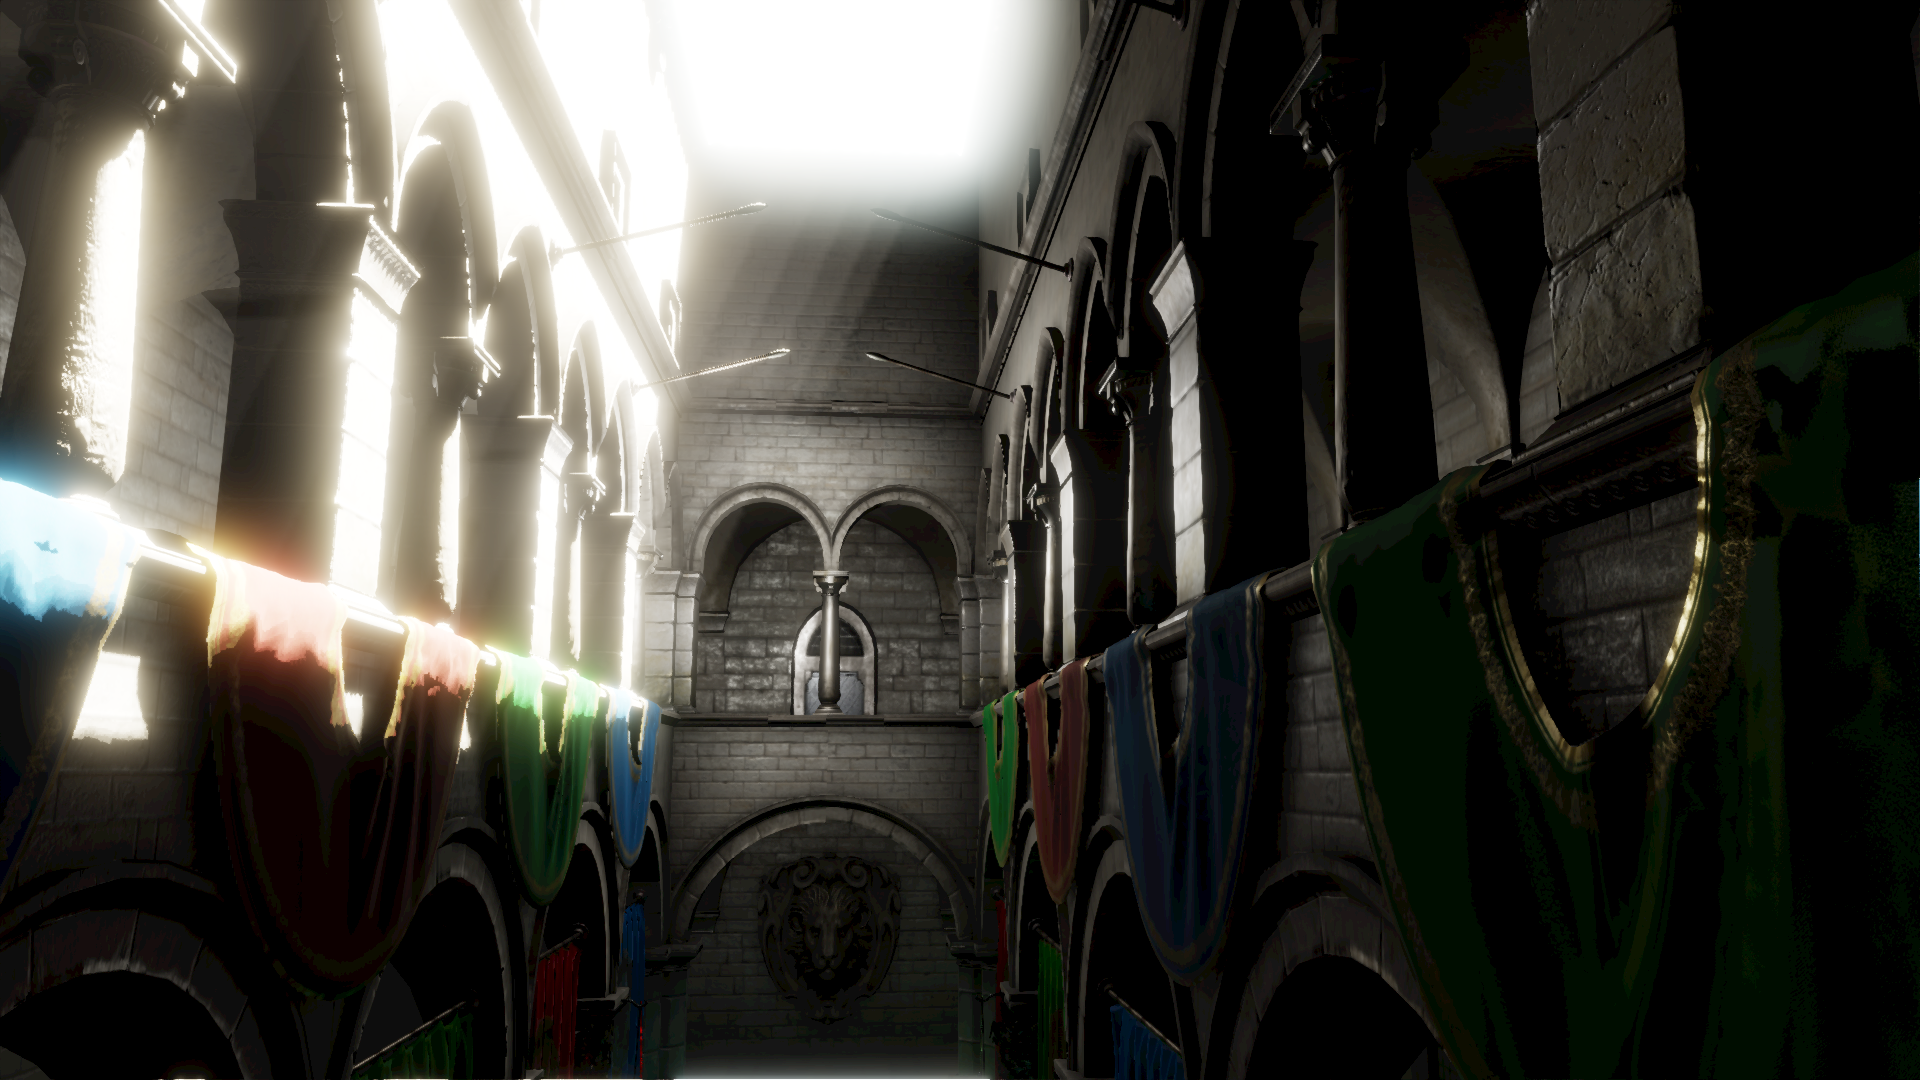
\includegraphics[width=\textwidth]{sunshaft_v2/halton/frame_000.png}
    \caption{优化后体积雾（\texttt{halton}：时域+深度保边+CSM PCF1）}
\end{subfigure}
\hfill
\begin{subfigure}{0.48\textwidth}
    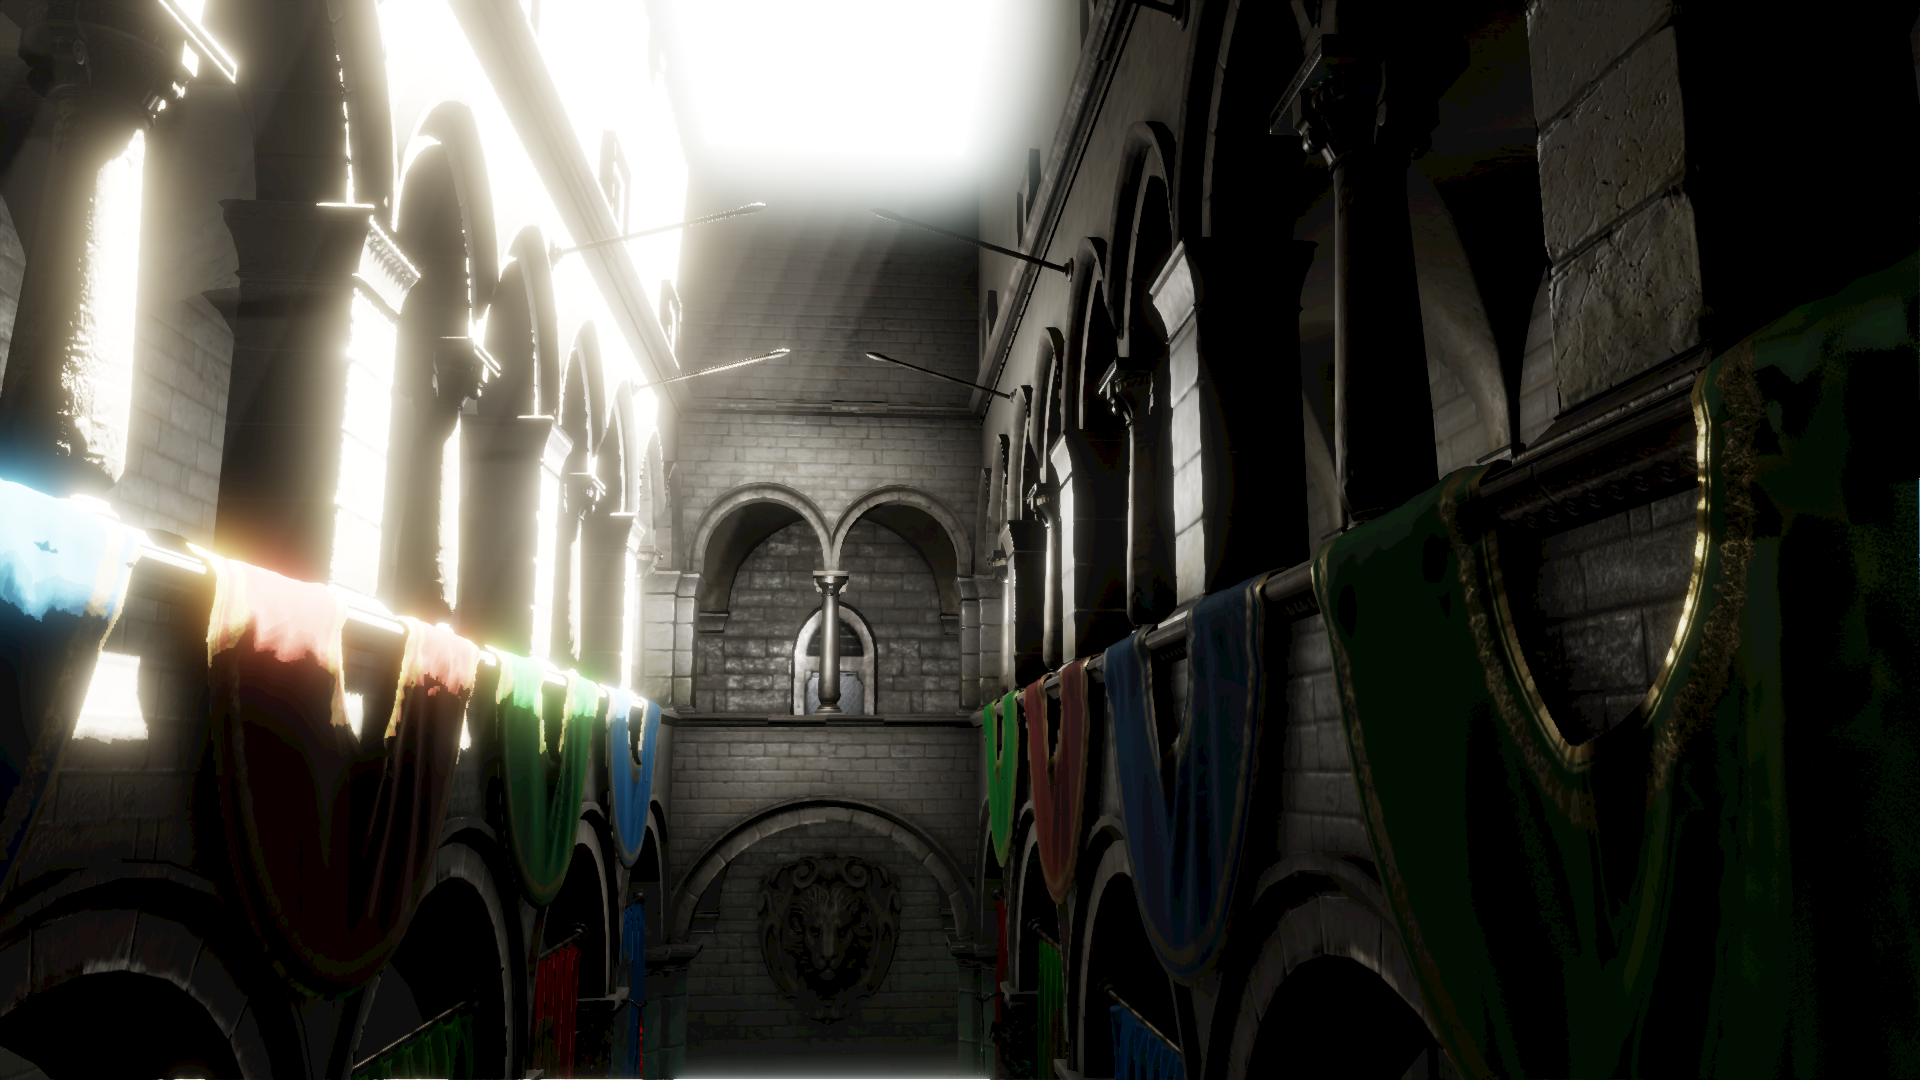
\includegraphics[width=\textwidth]{sunshaft_v2/fast_xy/frame_000.png}
    \caption{FAST 体积雾（\texttt{fast\_xy}：FAST XY 采样替换 Halton）}
\end{subfigure}
\caption{Sponza 光柱视角四种状态对比（轨迹起点 frame 0）。}
\label{fig:four-state-start}
\end{figure}

\subsection{测试环境}

\begin{table}[H]
\centering
\begin{tabular}{ll}
\toprule
项目 & 值 \\
\midrule
GPU & NVIDIA GeForce RTX 4060 Laptop GPU (8188 MiB) \\
CPU & Intel Core i7-13700H (14C/20T) \\
内存 & 32 GiB \\
RHI & Vulkan, API 1.4.325 \\
构建 & Debug, Clang 22.1.8 + Ninja \\
分辨率 & 1920$\times$1080 \\
场景 & Sponza (\texttt{Camera.001}) \\
Froxel 网格 & 320$\times$180$\times$64 = 3,686,400 个体素 \\
体积雾显存 & 自有资源 31.89\,MiB + FAST 噪声 0.50\,MiB = 32.39\,MiB \\
\bottomrule
\end{tabular}
\caption{测试环境配置}
\end{table}

\subsection{配置对比}

以下数据通过引擎内置 GPU Timestamp Scope 每秒采样获得。Benchmark 以固定时间步长（1/60s）运行，120 帧 warmup 后进入 90 帧轨迹，丢弃前 3 条记录取稳定值。

\textbf{关闭 Probe GI 的历史对照（Froxel 160$\times$90$\times$64）：}

\begin{table}[H]
\centering
\begin{tabular}{lrrl}
\toprule
配置 & GraphicsExec (ms) & FogTotal (ms) & 说明 \\
\midrule
Fog Off & 14.043 & 0.000 & 热态基线 \\
完整功能 (Halton) & 14.639 & 0.561 & Probe GI 关闭 \\
完整功能 (FAST XY) & 14.721 & 0.571 & Probe GI 关闭 \\
\bottomrule
\end{tabular}
\caption{历史对照数据（Probe GI 关闭）}
\end{table}

\textbf{本次本机实测（Froxel 320$\times$180$\times$64，Probe GI + VRC 开启）：}

\begin{table}[H]
\centering
\begin{tabular}{lrrr}
\toprule
配置 & GraphicsExec 均值 (ms) & FogTotal 均值 (ms) & StdDev (ms) \\
\midrule
Fog Off (基线) & $\sim$11.2 & --- & --- \\
完整功能 (Halton + Probe GI + VRC) & 17.173 & \textbf{6.508} & 0.183 \\
\bottomrule
\end{tabular}
\caption{本次本机实测数据}
\end{table}

> Froxel 网格从 160$\times$90$\times$64 升级到 320$\times$180$\times$64（4$\times$ 体素），且 Probe GI 注入从关闭变为开启。FogTotal 增大主要来自 Probe GI 注入开销。

\subsection{阶段分解}

以下为本次实测的逐 Pass GPU 时间分解（6 个一秒采样均值）：

\begin{table}[H]
\centering
\begin{tabular}{lrrr}
\toprule
阶段 & 均值 (ms) & 标准差 (ms) & FogTotal 占比 \\
\midrule
CSM 阴影采样 & 0.143 & 0.004 & 2.2\% \\
阴影时域滤波 & 0.104 & 0.014 & 1.6\% \\
\textbf{光照/CSM/ProbeGI 注入} & \textbf{5.760} & \textbf{0.193} & \textbf{88.5\%} \\
介质时域重投影 & 0.232 & 0.000 & 3.6\% \\
Beer-Lambert 积分 & 0.049 & 0.001 & 0.8\% \\
调试可视化 & 0.015 & 0.000 & 0.2\% \\
深度感知合成 & 0.203 & 0.021 & 3.1\% \\
VRC 稀疏更新 & 0.066 & 0.001 & 1.0\% \\
\midrule
\textbf{合计} & \textbf{6.508} & \textbf{0.183} & \textbf{100\%} \\
\bottomrule
\end{tabular}
\caption{本次实测阶段分解}
\end{table}

\subsection{VRC 开销验证}

VRC 稀疏更新在历史报告和本次实测中开销一致：

\begin{table}[H]
\centering
\begin{tabular}{lrll}
\toprule
数据来源 & VRC 更新 (ms) & Froxel 网格 & Probe GI \\
\midrule
历史报告 & 0.064 & 160$\times$90$\times$64 & 关闭 \\
本次实测 & 0.066 & 320$\times$180$\times$64 & 开启 \\
\bottomrule
\end{tabular}
\caption{VRC 开销验证}
\end{table}

VRC 开销不随 Froxel 分辨率或 Probe GI 状态变化。更新量受每帧 2 Brick 预算限制，不会随世界空间体积线性增长。VRC 双缓冲共占用 0.3125\,MiB 显存。

\subsection{性能结论}

\begin{enumerate}[label=\textbf{\arabic*.}]
    \item \textbf{Probe GI 注入是当前最大性能瓶颈。} 开启 Probe GI 后，Injection 从 0.196\,ms（关闭时）飙升至 5.760\,ms，占 FogTotal 的 88.5\%。每个 $4\times4\times4$ Froxel 工作组执行完整的 8 角点三线性 Probe 查询 + Ray Query 可见性测试，成本远超其余所有阶段之和。是后续主要优化方向。

    \item \textbf{VRC 以极低成本补全世界空间间接雾光。} 0.066\,ms GPU 时间和 0.3125\,MiB 显存，占 FogTotal 仅 1.0\%。两次独立测量（0.064 vs 0.066\,ms）证明其开销稳定，不受 Froxel 分辨率影响。

    \item \textbf{非 Injection 阶段开销合理。} CSM 阴影 (0.143\,ms)、介质时域 (0.232\,ms)、深度合成 (0.203\,ms) 等阶段在 4$\times$ Froxel 体素下总计约 0.75\,ms，与历史报告的 0.561\,ms（2$\times$ 粗网格）在量级上一致。

    \item \textbf{整帧 GPU 时间约 17.2\,ms（约 58 FPS）。} 其中体积雾占 6.5\,ms（37.8\%），是仅次于几何渲染的第二大开销。Probe GI 注入优化是提升帧率的最有效路径。
\end{enumerate}

\subsection{优化方向}

基于本次实测数据，后续性能优化应优先解决 Probe GI 注入瓶颈：

\begin{itemize}
    \item \textbf{查询缓存}：相邻 Froxel 工作组查询的 Probe 位置高度重叠，可用 LDS 或纹理缓存避免重复查询
    \item \textbf{降低查询频率}：每隔 N 帧更新一次 Probe GI 注入，中间帧使用历史值插值
    \item \textbf{降采样 Probe 查询}：在低频区域使用更粗的 Probe 层级，减少 8 角点查询为 1 角点
    \item \textbf{按需执行 Debug Visualize}：当前每帧 Dispatch 调试图，固定浪费 0.015\,ms，生产路径应只在选择调试输出时执行
\end{itemize}

% ================================================================
\section{结论与展望}
% ================================================================

\subsection{实验总结}

本次暑期课题研究在大约半个月的时间里，完成了从 MoerEngine 的开发环境部署与相关内容学习，到 MVP 体积雾的搭建，并进行了与 UE 的对齐；完成了适配 MoerEngine 的优化，最终完成了一个基础可用版本的体积雾，并在此基础上，进一步完成了两项扩展工作：

\textbf{FAST 采样论文适配}：选择了 Filter-Adapted Spatio-Temporal Sampling 论文进行工程化改造，将其与 Moer 的稳定网格语义、0.94 历史权重和 7-tap 邻域 Clamp 绑定。通过设计高对比度场景和未收敛场景（模拟相机切换）两组对照实验，量化了 FAST 与 Halton 在不同条件下的像素差异；

\textbf{自适应稀疏体积辐射缓存（VRC）}：复用 Moer 独有的动态稀疏 Probe GI 基础设施，构建了独立的世界空间介质辐射缓存，以 0.066\,ms GPU 开销和 0.3125\,MiB 显存的极低代价补全了 Froxel 网格无法覆盖的远处间接雾光。

最终通过引擎内置 GPU Timestamp Scope 完成了完整的性能实测，识别出 Probe GI 注入（5.76\,ms，占 FogTotal 88.5\%）是当前最大性能瓶颈，并给出了查询缓存、降采样等后续优化方向。

同时开发使用了 benchmark 工具，支持固定相机轨迹、逐帧截图、GIF 模式和多 preset 自动对照，为效果比对提供了良好的环境。

本次实践让我对 MoerEngine 与 VolumetricFog 的实现有了更深入的了解，为后续的学习和开发提供了坚实的基础。

\subsection{未来工作}

\begin{enumerate}[label=(\arabic*)]
    \item \textbf{优化 Probe GI 注入}：当前版本 Probe GI 注入开销过大，对整体性能表现造成了较高的影响，未来可考虑通过查询缓存、降采样等手段降低 Probe GI 注入开销。
    \item \textbf{相关论文适配}：继续研究更多最新的论文，尝试将深度学习内容加入到 MoerEngine 中，提升 MoerEngine 的性能。
\end{enumerate}

% ================================================================
\section*{附录：关键文件索引}
% ================================================================
\addcontentsline{toc}{section}{附录：关键文件索引}

\begin{longtable}{lp{8cm}}
\toprule
\textbf{类型} & \textbf{文件} \\
\midrule
\endhead
C++ Pass & \texttt{source/runtime/render/renderer/raster/VolumetricFogPass.cpp/h} \\
VRC 调度 & \texttt{source/runtime/render/renderer/raster/ProbeUpdatePass.h} \\
Benchmark & \texttt{source/runtime/render/renderer/raster/VolumetricFogBenchmark.cpp/h} \\
配置 & \texttt{source/runtime/render/renderer/raster/RasterConfig.h} (L342--423) \\
\midrule
InjectDensity & \texttt{shaders/pipelines/raster/volumetric\_fog/InjectDensity.hlsl} \\
ShadowVisibility & \texttt{shaders/pipelines/raster/volumetric\_fog/ShadowVisibility.hlsl} \\
Temporal & \texttt{shaders/pipelines/raster/volumetric\_fog/TemporalReprojection.hlsl} \\
Integrate & \texttt{shaders/pipelines/raster/volumetric\_fog/IntegrateScattering.hlsl} \\
Composite & \texttt{shaders/pipelines/raster/volumetric\_fog/CompositeVolumetricFog.hlsl} \\
VRC 核心 & \texttt{shaders/pipelines/raster/volumetric\_fog/VolumetricRadianceCache.hlsli} \\
VRC 更新 & \texttt{shaders/pipelines/raster/volumetric\_fog/UpdateRadianceCache.hlsl} \\
\midrule
FAST 资产 & \texttt{asset/textures/volumetric\_fog\_fast\_vector3\_gauss1\_exp006\_beta010\_64x64x32.rgba8} \\
\midrule
实施计划 & \texttt{docs/260714-VolumetricFogImplPlan.md} \\
研究方案 & \texttt{docs/260801-RecentVFogResearchAndMoerPlan.md} \\
性能报告 & \texttt{docs/260802-VolumetricFogPerformanceEval.md} \\
参数冻结 & \texttt{docs/260802-VolumetricFogBenchmark.md} \\
VRC 报告 & \texttt{docs/260803-AdaptiveSparseVRC.md} \\
\bottomrule
\end{longtable}

\end{document}
